\documentclass[12pt,letterpaper]{article}
\usepackage[margin=1in]{geometry}
\usepackage[english]{babel}
\usepackage [autostyle, english = american]{csquotes}
\MakeOuterQuote{"}
\usepackage[utf8x]{inputenc}
\usepackage{amsmath}
\usepackage{amssymb} 
\usepackage[retainorgcmds]{IEEEtrantools}
\usepackage{graphicx}
\usepackage{tabularx}
\usepackage{subfig}
\usepackage{kpfonts}    % for nice fonts
\usepackage{microtype} 
\usepackage{booktabs}   % for nice tables
\usepackage{bm}         % for bold math
\usepackage{listings}   % for inserting code
\usepackage{verbatim}   % useful for program listings
\usepackage{color}  
\usepackage[colorlinks=true, citecolor=black]{hyperref}
% use for hypertext
\usepackage[colorinlistoftodos]{todonotes}
\usepackage{natbib}
\usepackage{amssymb}
\usepackage{amsmath}
\usepackage{setspace}
\usepackage{caption}
\usepackage{float}
\newfloat{Equation}{htbp}{loa}
\usepackage{geometry}
\usepackage[compact]{titlesec}
\usepackage{makecell}
\usepackage{pdflscape}
\usepackage{chngcntr}


\setcounter{MaxMatrixCols}{10}
\geometry{letterpaper,tmargin=1in,bmargin=1in,lmargin=1.0in,rmargin=1.0in}
\hypersetup{urlcolor=black,citecolor=black,colorlinks=true,linkcolor=black,raiselinks=false,pdfstartview={XYZ null null 1.20}}
\linespread{1.5}
\setlength{\footnotesep}{0.7\baselineskip}
\setlength{\parindent}{24pt}

\newcolumntype{P}[1]{>{\centering\arraybackslash}p{#1}}
\newcolumntype{L}[1]{>{\hangindent=1em \raggedright \let\newline\\\arraybackslash}p{#1}}
%\newcolumntype{C}[1]{>{\centering\let\newline\\\arraybackslash\hspace{0pt}}m{#1}}
%\newcolumntype{R}[1]{>{\raggedleft\let\newline\\\arraybackslash\hspace{0pt}}m{#1}}


\newenvironment{nenumerate}{\enumerate\addtolength{\itemsep}{-3pt}}{\endenumerate}


\titlespacing{\section}{0pt}{10pt}{5pt}
\titlespacing{\subsection}{2pt}{8pt}{4pt}
\titlespacing{\subsubsection}{0pt}{10pt}{3pt}

\newtheorem{result}{Prediction}
\newtheorem{claim}{Claim}
\newtheorem{assumption}{Assumption}

\graphicspath{{"./graphs/"}{"./maps/"}}
\widowpenalty=10000

\begin{document}
\title{\vspace{-.8cm}Insurer Competition in the Age of Provider Consolidation:
The relationship between hospital and insurance competition in the ACA individual market\thanks{I thank Professors Colleen M. Grogan, Kotaro Yoshida and Victor O. Lima for all their guidance over the course of this project. I thank Professor Seema Jayachandran for her helpful commments. I thank the Dean's Fund and the Becker Friedman Institute for sponsoring this project.}}
\date{\vspace{.3cm}\today}
\author{\begin{tabular}{c}
 Jacob Toner Gosselin\end{tabular}}
\maketitle
\normalsize


\begin{abstract}\onehalfspacing{
\noindent This paper investigates the impact of hospital competition (or lack thereof) on insurer participation in the ACA's individual market. Using public data from CMS, and private data from the American Hospital Association (AHA), I construct the Herfindahl–Hirschman Index (HHI)  for hospital and insurer markets at the county-level in 34 of the 36 states using federally facilitated marketplaces, across 2015 and 2016 (hospital HHI is lagged by one year). I fit a linear model on 2063 counties across two years in these states, controlling for county-level covariates and fixed effects for year-"rating area" (a geographic designation created by the ACA,  which typically amounts to a collection of counties). I estimate my parameters using OLS. I find higher hospital HHI levels are associated with higher insurer HHI levels at a coefficient of .033, log linearized. I lay the groundwork for further analysis once more years of data are available, contributing to the existing literature by focusing on insurer competition rather than premium price as my primary outcome, leveraging "rating areas" for better model specification, and outlining a novel approach to hospital market HHI construction using hospital "radii" rather than pre-existing geographic bounds. }\end{abstract}

\DeclareGraphicsExtensions{.pdf,.tif}

\thispagestyle{empty}

\newpage \setcounter{page}{1}

\section*{Introduction}
Since the Affordable Care Act (ACA) came into effect in 2014, the state of its exchanges (regulated markets that allow individuals to buy coverage separate from their employer) has been closely studied as an indicator of the law's success.  Though these exchanges represent only a fraction of the insured population (roughly 4 percent, or 9 million individuals nationwide), they've adopted outsized political significance. In the past few years, diminishing competition on exchanges nationwide has sparked panic about these markets' sustainability \citep{cox_analysis_2015}. 

Qualitative studies have pointed to competition among healthcare providers as "essential to a robust and competitive insurer market" \citep{morrisey_five-state_2017}. Most quantitative work, however, has either ignored provider competition when looking at diminishing insurer choice,  or focused on how provider competition relates to insurer premiums, rather than participation, in ACA exchanges.

This paper seeks to fill this hole and lay a groundwork for future analysis once more years of data are generated. It is a "first go" at answering two questions: 1) How is competition between short term general hospitals related to competition on ACA exchanges, and 2) How robust is this relationship to regional variation and model specification? It adds to the literature by documenting a novel method of constructing hospital market HHI at the county-level and by illustrating how rating areas, a unique feature of ACA markets, allow for some control of intra-state geographic fixed effects, even with limited data. 

It is organized as follows: Section 1 reviews the relevant research on market dynamics in the ACA, and explains how my work fits into this existing literature; Section 2 goes over my data construction; Section 3 explains my model; Section 4 reviews my results; Section 5 explains the limitations of my model; Sections 6 and 7 discuss my results and their policy implications; and Section 8 outlines potential directions for future work. 

\section{Background}
By 2016, the third year of ACA exchanges' operation, it was clear that maintaining a healthy level of competition in these markets posed a greater challenge than anticipated.  Between 2015 and 2016, the percent of enrollees in the individual market with three or more insurers to choose from fell from 91 percent to 85 percent, and the average "benchmark" premium (the premium of the second lowest cost "silver" plan in a rating area) rose by 4.4 percent \citep{cox_analysis_2015}.

In response to these concerning trends, the Brookings Institution's Center for Health Policy commissioned a field study across multiple state exchanges in 2016 \citep{morrisey_five-state_2017}. Researchers interviewed stakeholders in California, Michigan, Florida, North Carolina, and Texas, and came to four major conclusions: (1) health insurance markets are local, meaning the success or failure of insurers, even national ones, are determined by local factors; (2) higher than expected claims cost were the source of much of the early turmoil in insurance markets; (3) there has been a substantial shift towards narrower networks of healthcare providers, as a way of forcing hospitals to compete for enrollees by reducing reimbursement rates; and (4) hospital and physician competition is "essential" for a robust and competitive insurer market. 

These conclusions were prescient, and confirmed by quantitative work in the years following, which found that local factors (rurality, demographics, health spending, and state policy environment) had a significant impact on the number of insurers participating in a given rating area, and that insurance plans offered on ACA exchanges had "narrow networks", i.e. insurers offered a less broad network of healthcare providers to consumers in ACA exchanges than they did in their employer plans \citep{griffith_diminishing_2018} \citep{haeder_narrow_2015} . The shift to narrow networks was predictable given ACA regulations, which prevented insurers from "competing" over enrollees as they had pre-2014, through practices like denial of coverage and medical underwriting. Instead, insurers on ACA exchanges competed over providers; they narrowed their networks, and forced hospitals and doctors to offer cheaper reimbursement rates to have their enrollees as patients. In practice, this approach produced promising results: \citet{dafny_narrow_2017} found that narrow network plans were 16 percent cheaper than their broad network counterparts, and that such plans reduced medical costs. 

While these characteristics of ACA exchanges imply a link between provider competition and insurer competition, this relationship has only just begun to be examined. \citet{scheffler_consolidation_2018} looked at the impact provider consolidation had on premiums in California's state run ACA exchange. They regressed the Herfindahl-Hirschman Index (HHI) of short term general hospitals, measuring horizontal consolidation, the percent of physicians contracting with hospitals, measuring vertical consolidation, and the HHI of insurers in a given marketplace on the benchmark premium across California's 19 rating areas, over 3 years (all independent variables were lagged by one year). They found that a 10 percent increase in hospital HHI was associated with a 1.8 percent increase in marketplace premiums, while a 10 percent increase in insurer HHI was associated with a 2 percent increase in premiums.

\citet{boozary_association_2019} expanded the work of \citet{scheffler_consolidation_2018} to a nationwide sample, producing similar results: rating areas with the highest levels of hospital market concentration had annual premiums that were, on average, 5 percent higher than those in the least concentrated areas. They concluded that the "likely explanation for higher premiums being found in areas of greater hospital concentration (and, indeed, the one consistent with prior literature) is related to market power and the ability to negotiate higher prices from insurers and other payers in these areas." \citep{boozary_association_2019}. 

Both papers provide compelling evidence that concentrated hospital markets result in higher negotiated rates for insurers, which are then passed off to consumers in the form of higher premiums. However, they are limited in two respects: 1) their models are specified at the "rating-area" level, and 2) premiums may not be the best reflection of consumer experience in ACA exchanges.

In regards to (1), geographic "rating-areas" are intra-state regions (typically collections of counties) within which insurers must set premiums uniformly on ACA exchanges. However, \textbf{insurers are allowed to pick and choose which counties within a rating area they want to offer their plans}. As \citet{fang_why_2020} observed, it is quite common for insurers to selectively enter counties within a rating area.

While county-level variation isn't particularly important when looking at premiums as a primary outcome (especially benchmark premiums, as both \citet{scheffler_consolidation_2018} and \citet{boozary_association_2019} did), when looking at insurer participation it is essential. Moreover, variation in insurer participation across rating areas provides a powerful tool for model specification; even in cross-sectional analysis, rating areas can be used to control for intra-state geographic fixed effects, mitigating the risk of omitted-variable bias.

In regards to (2), while prices are obviously a primary indicator of consumer experience, they are not the only metric to measure market health. This is especially true for ACA exchanges, a heavily subsidized market where the vast majority of consumers pay for their plans as a percent of income, and are therefore shielded from price hikes. Choice and competition (i.e. HHI) are thus equally worthwhile metrics to consider as outcomes. In addition, insurer competition can also influence premium prices, as found by \citet{scheffler_consolidation_2018}.  Thus, if hospital competition influences insurer participation, it can have a two-fold impact on premium prices: first raising premiums due to higher reimbursement rates, then raising premiums due to reduced insurer competition. 

\section{Data Construction}
To measure insurer HHI, I pulled issuer-level enrollment data from the Center for Medicare and Medicaid Services (CMS). This enrollment data is for all federally facilitated marketplaces (FFMs), i.e. ACA exchanges run by the federal government. It includes 36 states. I removed Alaska and Nebraska from my analysis, as their rating areas are not based on county borders. The enrollment data also withholds information on counties with 10 or less enrollees in a given plan, due to privacy concerns. Moreover, 147 counties are in single county rating-areas, and are thus excluded from my main model which controls for rating-area fixed effects (they are included in alternative specifications). In total, we are left with 4128 county-year combinations (see Figure A.5 in the Appendix for a map of counties covered, color-coded by region). 

My enrollment data is for 2015 and 2016; these years provide the most stable market conditions, as insurers already had a year of experience in ACA exchanges (2014) and former President Trump was not yet elected (2017-2018). I constructed my HHI measurement by calculating market share for each insurer in a given county as a percent of total enrollees, and summing the results. A histogram summarizing the resulting distribution can be seen in Figure 1.

\begin{figure}[!h]
\begin{center}
\caption{Insurer HHI Distribution}\label{Figure 1}
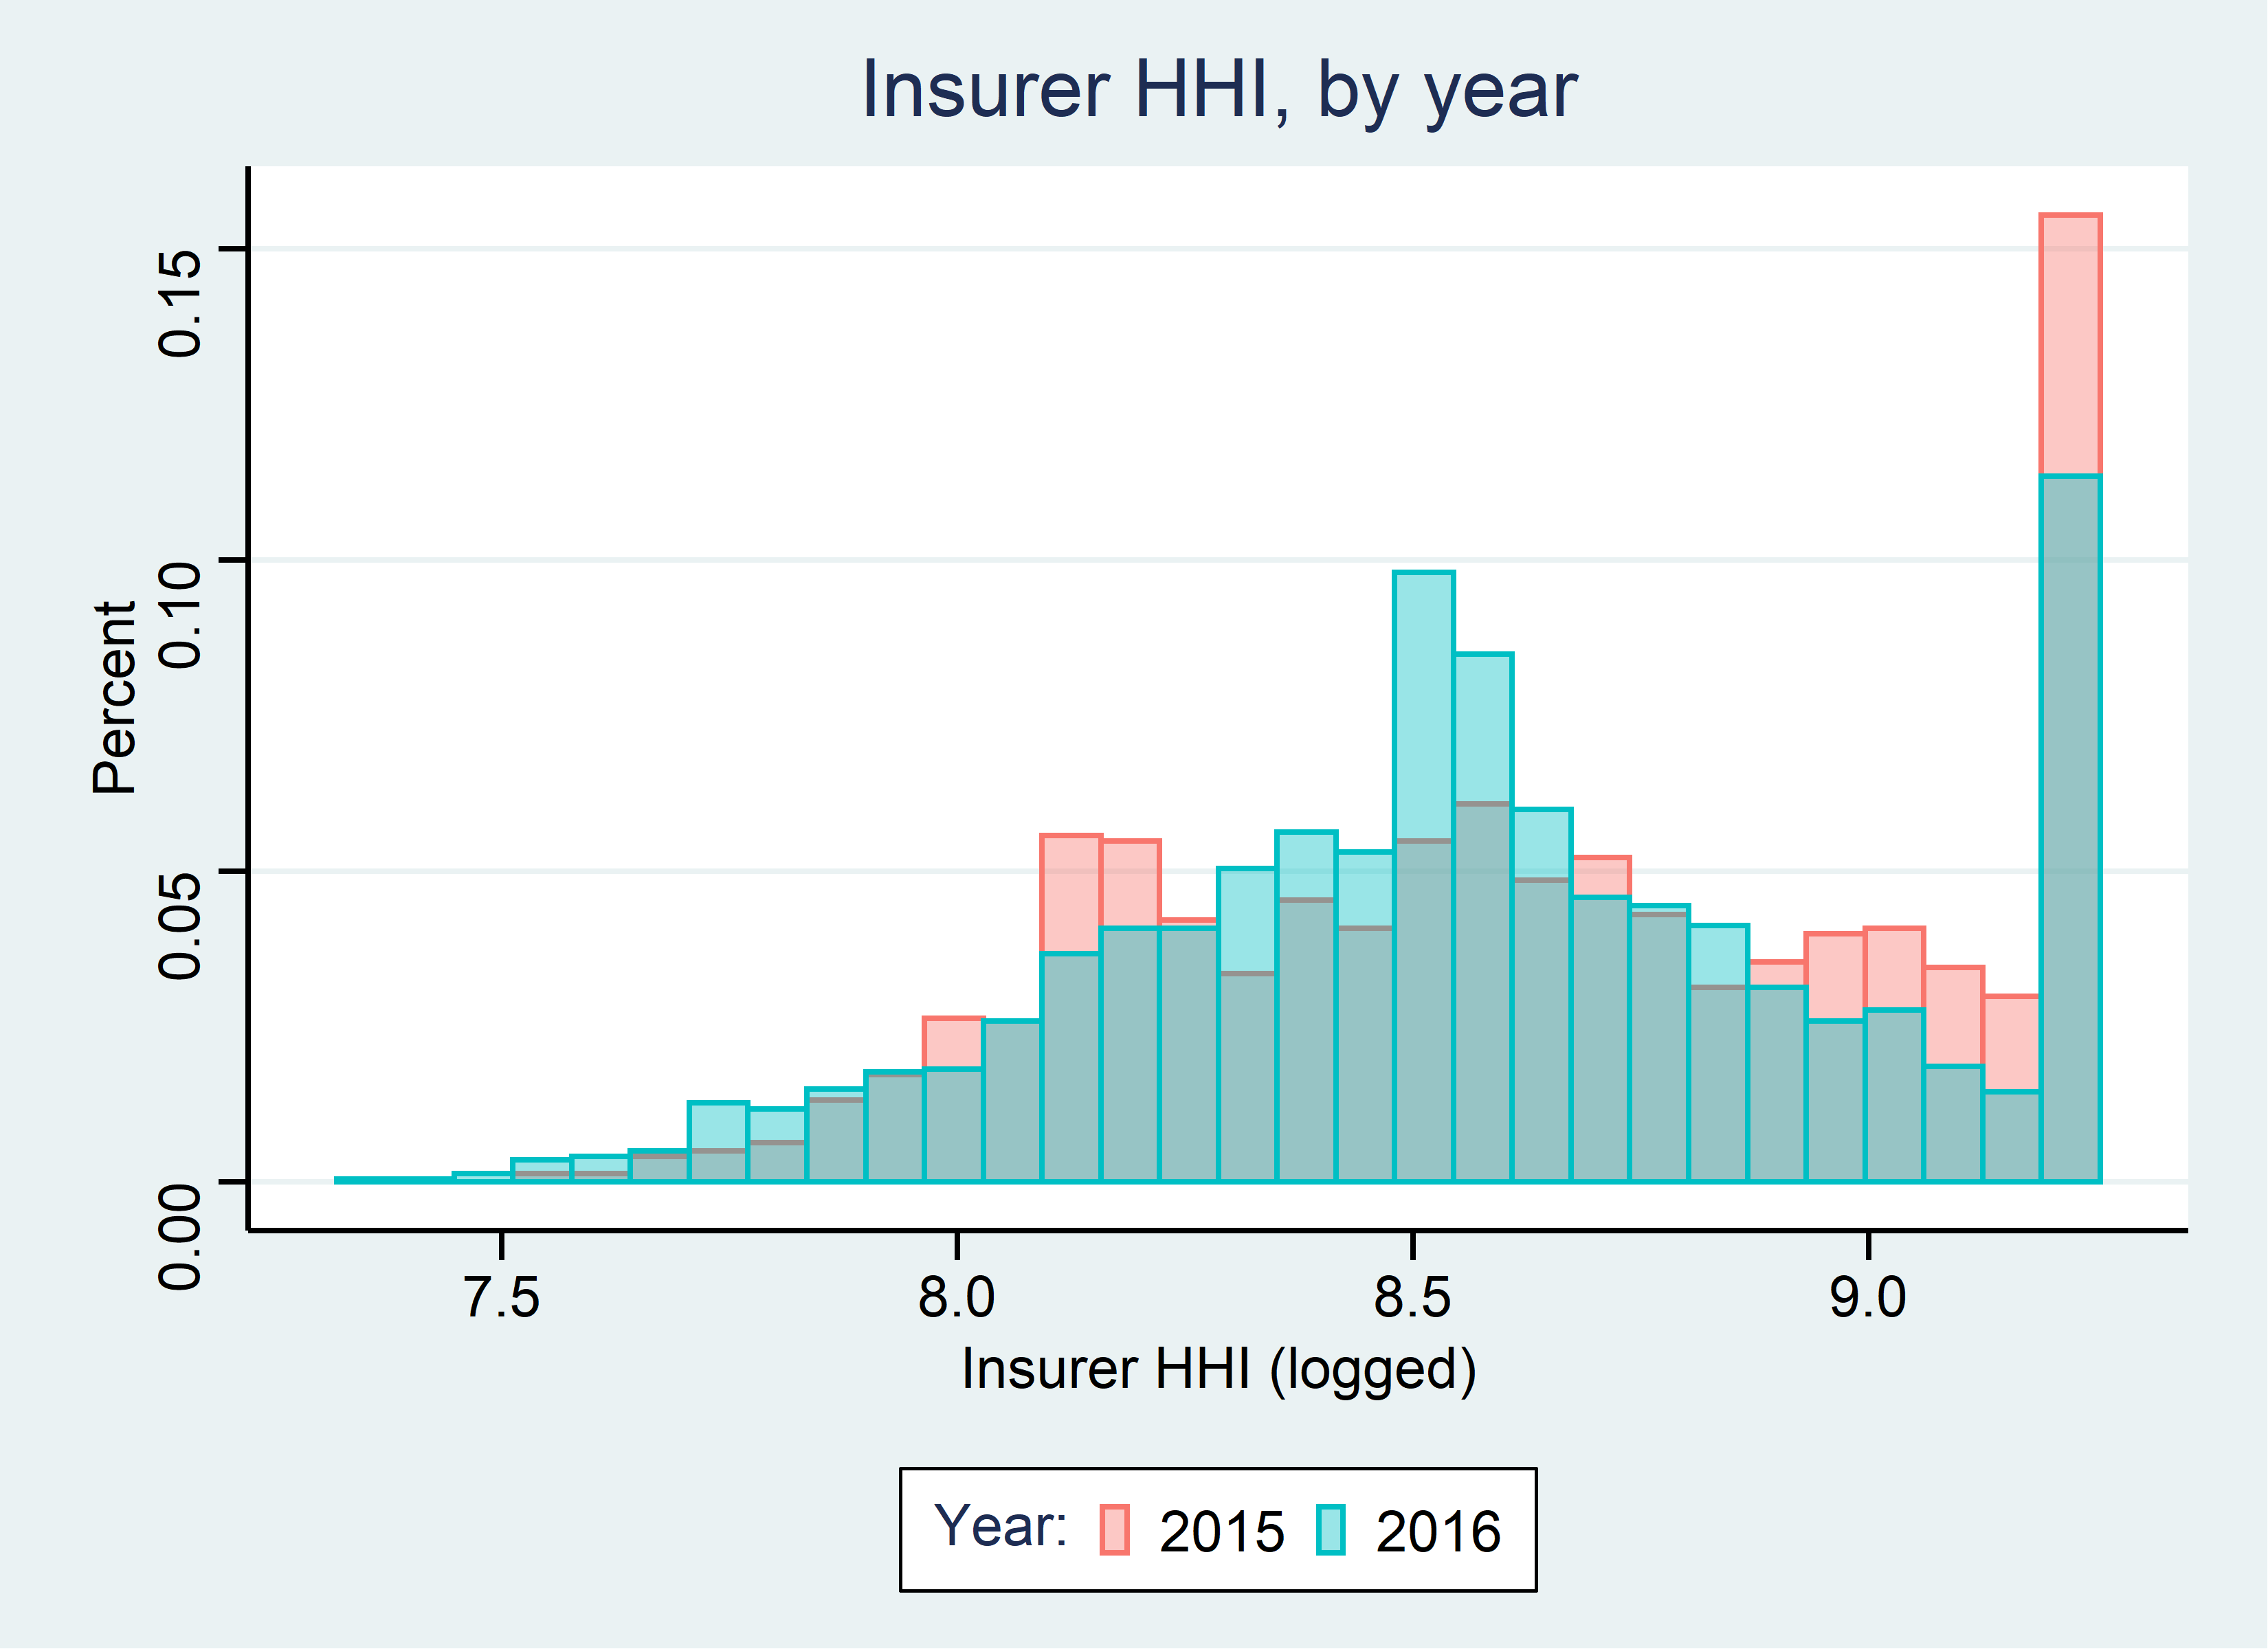
\includegraphics[height=4in,angle=0]{hist_year_insurerhhi.png}
\end{center}
\end{figure}

The rest of my variables are lagged by one year, since insurers decide on participating in a given county before November of the previous year. To measure provider competition, I used data from the American Hospital Association (AHA) Annual Survey on short term general care hospitals in 2014 and 2015. I use short term general care hospitals as this is the most common type of hospital nationwide, and the most relevant for insurers building provider networks on ACA exchanges (long term care facilities are usually used by Medicare or Medicaid enrollees). This is in line with the approach of \citet{scheffler_consolidation_2018}.  

\begin{figure}[!ht]
\begin{center}
\caption{Hospital HHI Distribution}\label{Figure 2}
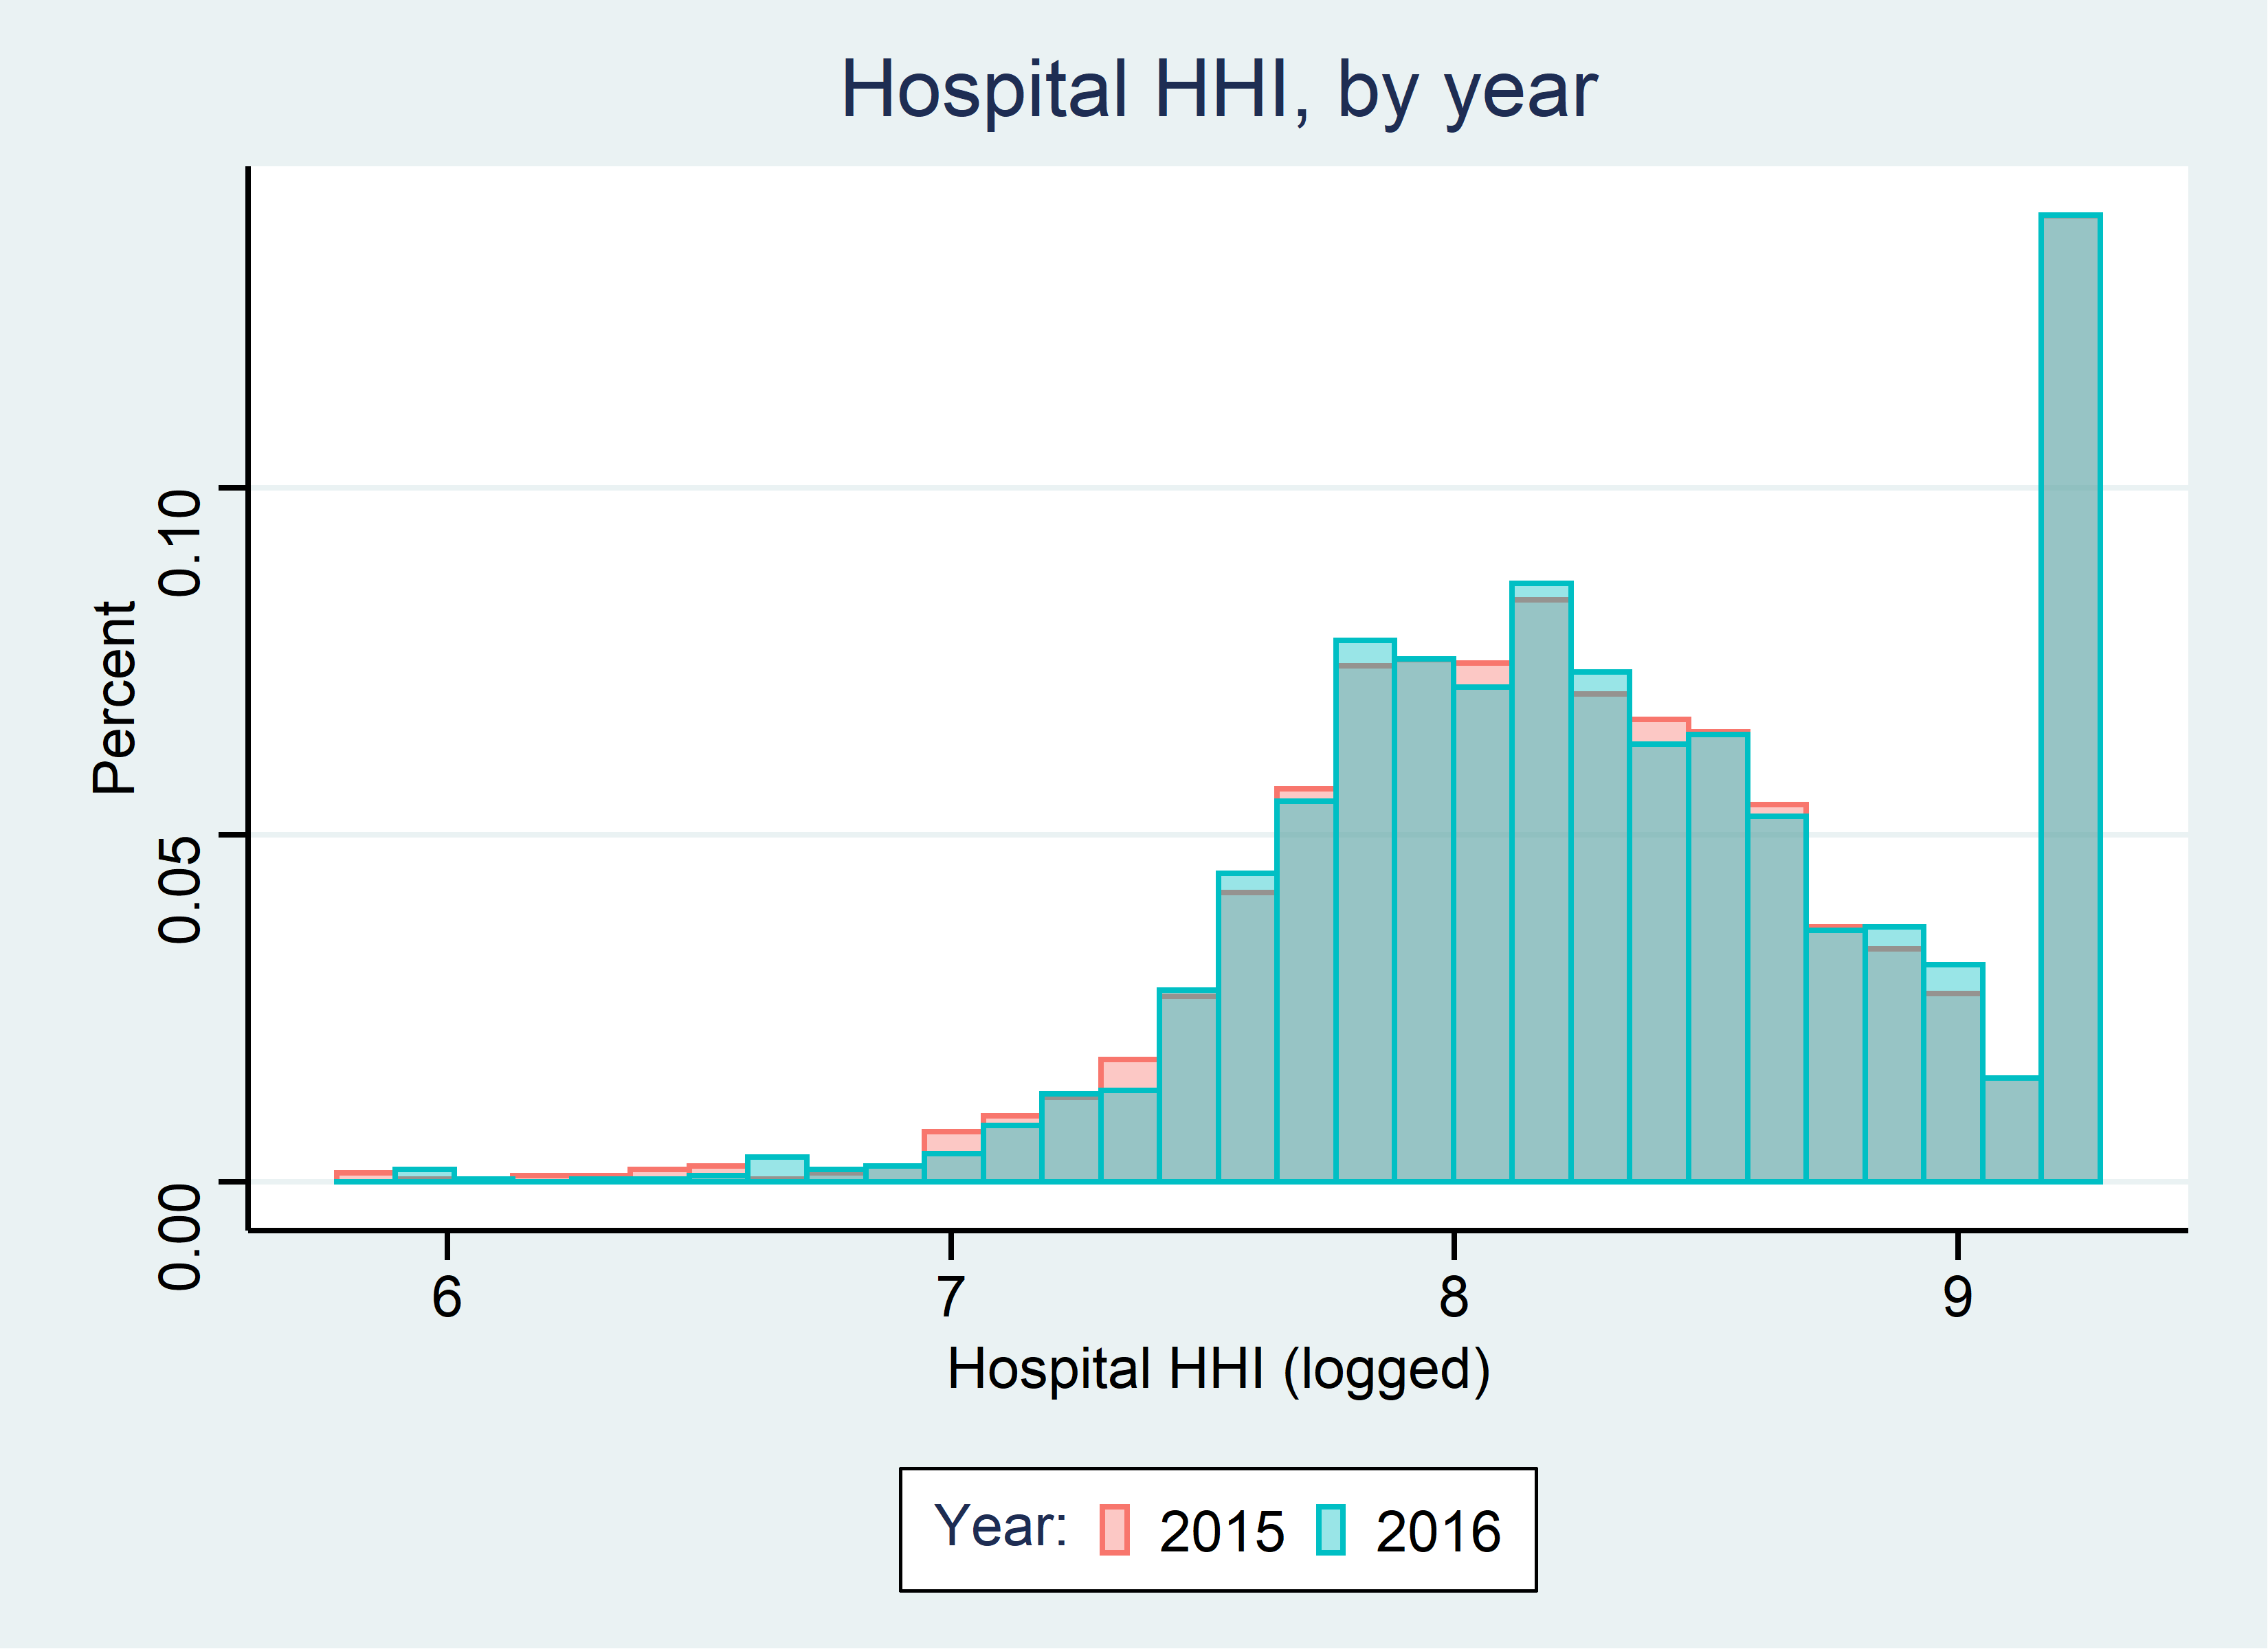
\includegraphics[height=4in,angle=0]{hist_year_hospitalhhi.png}
\end{center}
\end{figure}

While \citet{scheffler_consolidation_2018} and \citet{boozary_association_2019} constructed hospital HHI measurements using "rating-area" boundaries, I had to specify a county measure that allowed for intra-rating area variation. I chose not to use county boundaries, since they vary a great deal and can be too restrictive (many counties did not have a short-term hospital within their boundaries). Instead, I used the work of \citet{gresenz_updated_2004}, who found the "75 percent radii" for urban and rural hospitals, i.e. the boundary within which 75 percent of a hospital's admitted patients lived.  I draw radii around each of my hospitals based on their results (27.4 miles for hospitals in metro counties, 43.6 miles for hospitals in non-metro counties), and if the radius includes the centroid of a given county, I consider it part of that county's hospital market (a more extensive description of this approach, along with robustness checks for radii, can be found in the Appendix). From their, I construct hospital HHI in the typical fashion, using annual admissions as a measure of market share. There are 109 counties with no hospitals in their market; I assign these counties an HHI of 10000 and include a dummy variable for these "empty counties" as a control in my model. The distribution of the resulting HHIs can be seen in Figure 2. 

I control for all variables found to be significant in \citet{griffith_diminishing_2018}, and add a few controls of my own for good measure (see \hyperref[Table 1]{Table 1}).  My main model controls for rating area-year fixed effects, and therefore does not include any state-level covariates.  At the county level, I control for population demographics, poverty rate, and mortality rate using data from the Census Bureau's American Community Survey. I control for rurality using the 2013 Rural-Urban Continuum Codes (RUCC) assigned by the US Department of Agriculture Economic Research Service. I control for Medicare spending per capita using data from CMS.  I specify an additional model with no place-based fixed effects, and in this model I control for state policy environment using data from the National Bureau of State Legislatures (NBSL), Medicaid expansion status using data from the Kaiser Family Foundation (KFF), and average Medical Loss Ratio (MLR) rebate per capita using data from CMS (these are rebates paid by insurers when their medical claims cost is too low). A list of my variables and their source can be seen in Table 1, and summary statistics can be seen in Table 2. 

\vspace{1cm}

\begin{table}[H]
\caption{Control variables} \label{Table 1}
\centering
\begin{tabular}{l l l}
\toprule
\textbf{Variables} & \textbf{Geographic Level} & \textbf{Source}\\
\midrule
State Policy Environment & State & NBSL \\
Medicaid Expansion Status & State & KFF \\
Average MLR Rebate & State & CMS \\
Insurer HHI & County & CMS \\
Hospital HHI & County & AHA \\
Population Demographics & County & Census\\
Rurality & County & DOA\\
Medicare Spending & County & CMS \\
\bottomrule
\end{tabular}
\end{table} 

\newpage
\newgeometry{margin=1cm}
\begin{landscape}
\begin{table}[!h]
\scriptsize
	\caption{Summary Statistics}
	\centering
	
\begin{tabular}[t]{lcccccccccc}
\toprule
\multicolumn{1}{c}{} & \multicolumn{1}{c}{} & \multicolumn{2}{c}{Year} & \multicolumn{3}{c}{Rurality} & \multicolumn{4}{c}{Region} \\
\cmidrule(l{3pt}r{3pt}){3-4} \cmidrule(l{3pt}r{3pt}){5-7} \cmidrule(l{3pt}r{3pt}){8-11}
Variable & Overall & 2015 & 2016 & RUCC codes 1-3 & RUCC codes 4-6 & RUCC codes 7-9 & Northeast & North Central & South & West\\
\midrule
Number of Observations & 4128 & 2065 & 2063 & 1386 & 1260 & 1482 & 228 & 1729 & 1803 & 368\\
\addlinespace
Insurer HHI & \makecell[t]{5939.794\\{[}2359.088{]}} & \makecell[t]{6184.083\\{[}2442.054{]}} & \makecell[t]{5695.267\\{[}2247.153{]}} & \makecell[t]{5212.473\\{[}2225.781{]}} & \makecell[t]{5961.104\\{[}2366.917{]}} & \makecell[t]{6601.882\\{[}2275.705{]}} & \makecell[t]{5146.401\\{[}1549.223{]}} & \makecell[t]{5149.277\\{[}2073.401{]}} & \makecell[t]{6912.196\\{[}2355.398{]}} & \makecell[t]{5381.25\\{[}2307.157{]}}\\
\addlinespace
Hospital HHI & \makecell[t]{4734.51\\{[}2748.011{]}} & \makecell[t]{4722.359\\{[}2751.891{]}} & \makecell[t]{4746.673\\{[}2744.735{]}} & \makecell[t]{3555.38\\{[}2057.077{]}} & \makecell[t]{4508.93\\{[}2421.215{]}} & \makecell[t]{6029.047\\{[}3013.504{]}} & \makecell[t]{2940.513\\{[}2018.227{]}} & \makecell[t]{4659.111\\{[}2640.162{]}} & \makecell[t]{4284.685\\{[}2341.177{]}} & \makecell[t]{8404.155\\{[}2478.642{]}}\\
\addlinespace
Number of Insurers & \makecell[t]{3.483\\{[}1.823{]}} & \makecell[t]{3.559\\{[}1.866{]}} & \makecell[t]{3.406\\{[}1.775{]}} & \makecell[t]{4.283\\{[}2.123{]}} & \makecell[t]{3.433\\{[}1.716{]}} & \makecell[t]{2.777\\{[}1.199{]}} & \makecell[t]{5.145\\{[}1.487{]}} & \makecell[t]{4.002\\{[}1.906{]}} & \makecell[t]{2.713\\{[}1.399{]}} & \makecell[t]{3.783\\{[}1.81{]}}\\
\addlinespace
Number of ind. Hospitals & \makecell[t]{6.261\\{[}8.688{]}} & \makecell[t]{6.284\\{[}8.846{]}} & \makecell[t]{6.238\\{[}8.528{]}} & \makecell[t]{10.254\\{[}13.569{]}} & \makecell[t]{5.207\\{[}2.938{]}} & \makecell[t]{3.422\\{[}2.627{]}} & \makecell[t]{19.654\\{[}29.163{]}} & \makecell[t]{5.652\\{[}4.293{]}} & \makecell[t]{6.106\\{[}4.441{]}} & \makecell[t]{1.582\\{[}1.967{]}}\\
\addlinespace
Number of Hospitals & \makecell[t]{7.562\\{[}11.474{]}} & \makecell[t]{7.544\\{[}11.548{]}} & \makecell[t]{7.579\\{[}11.403{]}} & \makecell[t]{13.079\\{[}17.998{]}} & \makecell[t]{5.879\\{[}3.42{]}} & \makecell[t]{3.832\\{[}3.032{]}} & \makecell[t]{24.539\\{[}38.313{]}} & \makecell[t]{6.796\\{[}6.043{]}} & \makecell[t]{7.301\\{[}6.015{]}} & \makecell[t]{1.913\\{[}2.967{]}}\\
\addlinespace
No Hospitals & \makecell[t]{0.05\\{[}0.217{]}} & \makecell[t]{0.049\\{[}0.217{]}} & \makecell[t]{0.05\\{[}0.218{]}} & \makecell[t]{0.015\\{[}0.122{]}} & \makecell[t]{0.025\\{[}0.155{]}} & \makecell[t]{0.103\\{[}0.304{]}} & \makecell[t]{0\\{[}0{]}} & \makecell[t]{0.031\\{[}0.174{]}} & \makecell[t]{0.027\\{[}0.161{]}} & \makecell[t]{0.28\\{[}0.45{]}}\\
\addlinespace
Poverty rate & \makecell[t]{16.493\\{[}6.358{]}} & \makecell[t]{16.563\\{[}6.324{]}} & \makecell[t]{16.424\\{[}6.393{]}} & \makecell[t]{14.66\\{[}5.608{]}} & \makecell[t]{18.157\\{[}5.961{]}} & \makecell[t]{16.793\\{[}6.888{]}} & \makecell[t]{12.687\\{[}3.728{]}} & \makecell[t]{14.444\\{[}5.383{]}} & \makecell[t]{19.04\\{[}6.592{]}} & \makecell[t]{16.002\\{[}5.938{]}}\\
\addlinespace
Median age & \makecell[t]{41.014\\{[}5.135{]}} & \makecell[t]{40.948\\{[}5.104{]}} & \makecell[t]{41.079\\{[}5.165{]}} & \makecell[t]{39.282\\{[}4.36{]}} & \makecell[t]{40.231\\{[}4.51{]}} & \makecell[t]{43.298\\{[}5.463{]}} & \makecell[t]{42.522\\{[}3.438{]}} & \makecell[t]{41.633\\{[}4.989{]}} & \makecell[t]{40.145\\{[}4.877{]}} & \makecell[t]{41.425\\{[}6.934{]}}\\
\addlinespace
Percent white & \makecell[t]{0.85\\{[}0.156{]}} & \makecell[t]{0.851\\{[}0.155{]}} & \makecell[t]{0.849\\{[}0.156{]}} & \makecell[t]{0.831\\{[}0.143{]}} & \makecell[t]{0.852\\{[}0.155{]}} & \makecell[t]{0.866\\{[}0.166{]}} & \makecell[t]{0.888\\{[}0.12{]}} & \makecell[t]{0.919\\{[}0.1{]}} & \makecell[t]{0.774\\{[}0.174{]}} & \makecell[t]{0.876\\{[}0.131{]}}\\
\addlinespace
Percent Black & \makecell[t]{0.083\\{[}0.138{]}} & \makecell[t]{0.083\\{[}0.138{]}} & \makecell[t]{0.083\\{[}0.138{]}} & \makecell[t]{0.101\\{[}0.127{]}} & \makecell[t]{0.083\\{[}0.14{]}} & \makecell[t]{0.065\\{[}0.143{]}} & \makecell[t]{0.051\\{[}0.073{]}} & \makecell[t]{0.026\\{[}0.046{]}} & \makecell[t]{0.156\\{[}0.176{]}} & \makecell[t]{0.008\\{[}0.012{]}}\\
\addlinespace
Percent Native & \makecell[t]{0.033\\{[}0.007{]}} & \makecell[t]{0.033\\{[}0.007{]}} & \makecell[t]{0.033\\{[}0.007{]}} & \makecell[t]{0.033\\{[}0.006{]}} & \makecell[t]{0.033\\{[}0.006{]}} & \makecell[t]{0.031\\{[}0.009{]}} & \makecell[t]{0.029\\{[}0.004{]}} & \makecell[t]{0.033\\{[}0.006{]}} & \makecell[t]{0.033\\{[}0.007{]}} & \makecell[t]{0.033\\{[}0.01{]}}\\
\addlinespace
Medicare costs per-capita & \makecell[t]{9071.836\\{[}1305.533{]}} & \makecell[t]{8933.924\\{[}1292.173{]}} & \makecell[t]{9209.881\\{[}1304.557{]}} & \makecell[t]{9217.105\\{[}1157.74{]}} & \makecell[t]{9078.77\\{[}1153.951{]}} & \makecell[t]{8930.08\\{[}1524.535{]}} & \makecell[t]{9627.558\\{[}1230.387{]}} & \makecell[t]{8858.319\\{[}1122.542{]}} & \makecell[t]{9442.501\\{[}1322.306{]}} & \makecell[t]{7914.648\\{[}1134.67{]}}\\
\addlinespace
Counties per rating area & \makecell[t]{29.614\\{[}46.345{]}} & \makecell[t]{29.646\\{[}46.396{]}} & \makecell[t]{29.583\\{[}46.306{]}} & \makecell[t]{11.293\\{[}19.094{]}} & \makecell[t]{37.098\\{[}55.57{]}} & \makecell[t]{40.386\\{[}50.412{]}} & \makecell[t]{10.456\\{[}5.742{]}} & \makecell[t]{13.918\\{[}10.639{]}} & \makecell[t]{49.405\\{[}63.828{]}} & \makecell[t]{18.269\\{[}12.406{]}}\\
\addlinespace
Insurer "selective entry" rate & \makecell[t]{0.429\\{[}0.495{]}} & \makecell[t]{0.457\\{[}0.498{]}} & \makecell[t]{0.4\\{[}0.49{]}} & \makecell[t]{0.356\\{[}0.479{]}} & \makecell[t]{0.497\\{[}0.5{]}} & \makecell[t]{0.438\\{[}0.496{]}} & \makecell[t]{0.346\\{[}0.477{]}} & \makecell[t]{0.387\\{[}0.487{]}} & \makecell[t]{0.519\\{[}0.5{]}} & \makecell[t]{0.231\\{[}0.422{]}}\\
\addlinespace
Expanded Medicaid & \makecell[t]{0.372\\{[}0.483{]}} & \makecell[t]{0.356\\{[}0.479{]}} & \makecell[t]{0.388\\{[}0.487{]}} & \makecell[t]{0.374\\{[}0.484{]}} & \makecell[t]{0.388\\{[}0.488{]}} & \makecell[t]{0.357\\{[}0.479{]}} & \makecell[t]{0.566\\{[}0.497{]}} & \makecell[t]{0.592\\{[}0.492{]}} & \makecell[t]{0.063\\{[}0.243{]}} & \makecell[t]{0.734\\{[}0.443{]}}\\
\addlinespace
MLR rebate & \makecell[t]{164.418\\{[}179.749{]}} & \makecell[t]{136.488\\{[}144.16{]}} & \makecell[t]{192.376\\{[}205.673{]}} & \makecell[t]{160.416\\{[}173.055{]}} & \makecell[t]{174.31\\{[}186.62{]}} & \makecell[t]{159.752\\{[}179.728{]}} & \makecell[t]{86.004\\{[}64.616{]}} & \makecell[t]{97.307\\{[}111.67{]}} & \makecell[t]{255.769\\{[}209.818{]}} & \makecell[t]{80.747\\{[}113.212{]}}\\
\addlinespace
Republican state govt. & \makecell[t]{0.688\\{[}0.464{]}} & \makecell[t]{0.687\\{[}0.464{]}} & \makecell[t]{0.688\\{[}0.463{]}} & \makecell[t]{0.685\\{[}0.465{]}} & \makecell[t]{0.7\\{[}0.458{]}} & \makecell[t]{0.679\\{[}0.467{]}} & \makecell[t]{0.588\\{[}0.493{]}} & \makecell[t]{0.637\\{[}0.481{]}} & \makecell[t]{0.835\\{[}0.372{]}} & \makecell[t]{0.266\\{[}0.443{]}}\\
\bottomrule
\end{tabular}

\end{table}
\flushleft \footnotesize{Notes: Table reports variable means and standard deviations. Each observation is a county-year combination (i.e. Cook County in 2015). Counties in single-county rating areas are excluded.}
\end{landscape}
\restoregeometry

\section{Model}

Though I have data on counties over time, because I am limited to two years of data I do not do a straightforward panel regression. Instead, my approach is better described as a cross-sectional analysis, pooling two years of data to enlarge sample size, while controlling for the fixed effects of each rating area/year combination. I see this analysis as a "first-go" at assessing the relationship between hospital and insurer competition on ACA exchanges, laying the groundwork for an eventual panel regression once there are enough years of data.

I estimate the following linear model using ordinary least squares, with one observation per county-year combination (i.e. Cook County in 2015).
\\
\begingroup
\captionof{Equation}{Main model}
\vspace{-1.5cm}
\begin{equation}
\makebox[\textwidth]{%
$\begin{aligned}
Y_{i,t} = \beta_0 + \beta_1HospHHI_{i,t-1} +
\lambda\textbf{X}_{i,t-1} + \gamma_{ra_i, t} + \epsilon_{i,t} \notag \end{aligned}$}
\end{equation} 
\endgroup

$Y_{i,t}$ is insurer HHI (logged) in county $i$ in year $t$. $HospHHI_{i, t-1}$ is hospital HHI (logged) in county $i$ in year $t-1$ (as mentioned before, I lag my variable of interest and county controls by one year). $\textbf{X}_{i, t-1}$ is a vector of controls for county $i$ at time $t-1$ (this vector includes a binary for if the county has no hospitals in its market, which, as mentioned above, only occurs in 4.7 percent of counties). $\gamma_{ra_i, t}$ represent rating area-year fixed effects, i.e. controls for each rating area/year combination. Thus, $\beta_1$ represents the percent increase in insurer HHI associated with a 1 percent increase in hospital HHI, controlling for county level covariates, empty hospital markets, and rating area-year fixed effects.

I also specify two variations of my main model: one in line with the findings of \citet{boozary_association_2019}, and one in line with the findings of \citet{griffith_diminishing_2018}. In the former, I replace my rating area-year fixed effects ($\gamma_{ra_i, t}$) with state-year fixed effects ($\gamma_{st_i, t}$). This is similar to the model used in \citet{boozary_association_2019}, the difference being how I define my dependent variable (insurer HHI) and my variable of interest (hospital HHI).   
\\
\begingroup
\captionof{Equation}{\citet{boozary_association_2019}}
\vspace{-1.5cm}
\begin{equation}
\makebox[\textwidth]{%
$\begin{aligned}
Y_{i,t} = \beta_0 + \beta_1HospHHI_{i,t-1} +
\lambda\textbf{X}_{i,t-1} + \gamma_{st_i, t} + \epsilon_{i,t}  \notag \end{aligned}$}
\end{equation} 
\endgroup

In the latter, I drop my place-based fixed effects altogether and instead add a vector of state level covariates in line with \citet{griffith_diminishing_2018} ($\textbf{Z}_{i, t-1}$). I also add time fixed effects ($\tau_t$), i.e. a control for year (this effect is absorbed by our rating area-year/state-year fixed effects in the other two models).  
\\
\begingroup
\captionof{Equation}{\citet{griffith_diminishing_2018}}
\vspace{-1.5cm}
\begin{equation}
\makebox[\textwidth]{%
$\begin{aligned}
Y_{i,t} = \beta_0 + \beta_1HospHHI_{i,t-1} +
\lambda\textbf{X}_{i,t-1} + \zeta\textbf{Z}_{i,t-1} + \tau_t + \epsilon_{i,t} \notag \end{aligned}$}
\end{equation} 
\endgroup

These models offer more variation for OLS to exploit (we can now make comparisons across rating areas, rather than just within them). It also allows us to incorporate the aforementioned 147 counties in single county rating areas. On the other hand, the risk of omitted variable bias is higher. 

I cluster my standard errors at the county level, since my pooled two years of data are over the same set of counties \citep{abadie_when_2017}.

\section{Results}

I fit all three models on my overall dataset in Table 3, and fit my main model on subsets of the data by region and rurality in Table 4 and Table 5 respectively. All coefficients of interest are the result of a log to log comparison, so they can be interpreted as a percent to percent relationship. 

My overall coefficient of interest in my main model is .033; in other words, a 10 percent increase in hospital HHI is associated with a .33 percent increase in insurer HHI. In my alternative models (\citet{boozary_association_2019} and \citet{griffith_diminishing_2018}) my coefficients are .045 and .054, respectively. My coefficient of interest is significant at $p<.01$ in all models, and the coefficient increases as I relax my fixed effects (i.e. allow for more variation to be used in my coefficient estimate, with a higher risk of endogeneity). Going forward I will only consider my main model, as I believe it is best specified (it has the most rigorous controls, and therefore the lowest likelihood of omitted variable bias).

While my coefficients are small, the narrow distribution of insurer HHI (see Figure 1) implies humble coefficients across the board: there simply isn't much variation to be explained, especially when controlling for time and place-based fixed effects (95 percent of logged insurer HHI is between [8.20, 9.02]; to put that another way, 61 percent of counties across my two years of data had 3 or less insurers in their market). This trend carries over to my control variables: all county level covariates are insignificant in my main model except poverty rate, with a coefficient of .0017, and rurality (measured by RUCC) with a coefficient of .013. 

\begin{table}[!h]
\centering
\caption{Main results}

% Table created by stargazer v.5.2.2 by Marek Hlavac, Harvard University. E-mail: hlavac at fas.harvard.edu
% Date and time: Mon, Mar 15, 2021 - 11:56:54 PM
\begingroup 
\scriptsize 
\begin{tabular}{@{\extracolsep{5pt}}lccc} 
\\[-1.8ex]\hline 
\hline \\[-1.8ex] 
 & \multicolumn{3}{c}{\textit{Dependent variable:}} \\ 
\cline{2-4} 
\\[-1.8ex] & \multicolumn{3}{c}{Insurer HHI (logged)} \\ 
 & Main model & Boozary et al. (2019) & Griffith et al. (2018) \\ 
\\[-1.8ex] & (1) & (2) & (3)\\ 
\hline \\[-1.8ex] 
 Hospital HHI (logged) & 0.033$^{***}$ & 0.045$^{***}$ & 0.054$^{***}$ \\ 
  & (0.008) & (0.009) & (0.011) \\ 
  & & & \\ 
 No hospitals in market & 0.018 & 0.035 & 0.039 \\ 
  & (0.015) & (0.021) & (0.028) \\ 
  & & & \\ 
 Rurality (RUCC code) & 0.013$^{***}$ & 0.033$^{***}$ & 0.040$^{***}$ \\ 
  & (0.002) & (0.002) & (0.002) \\ 
  & & & \\ 
 Year &  &  & $-$0.074$^{***}$ \\ 
  &  &  & (0.011) \\ 
  & & & \\ 
\hline \\[-1.8ex] 
Observations & 4,128 & 4,410 & 4,410 \\ 
R$^{2}$ & 0.825 & 0.581 & 0.214 \\ 
Adjusted R$^{2}$ & 0.803 & 0.574 & 0.211 \\ 
Residual Std. Error & 0.182 (df = 3665) & 0.266 (df = 4339) & 0.362 (df = 4395) \\ 
F Statistic & 37.354$^{***}$ (df = 462; 3665) & 85.784$^{***}$ (df = 70; 4339) & 85.267$^{***}$ (df = 14; 4395) \\ 
\hline 
\hline \\[-1.8ex] 
\textit{Note:}  & \multicolumn{3}{r}{$^{*}$p$<$0.1; $^{**}$p$<$0.05; $^{***}$p$<$0.01} \\ 
 & \multicolumn{3}{r}{Controlling for rating area-year fixed effects in (1) and state-year fixed effects in (2).} \\ 
 & \multicolumn{3}{r}{Controlling for county/state covariates where appropriate.} \\ 
\end{tabular} 
\endgroup 

\end{table}

Exponentiating my coefficients, we see that a 1-point increase in the 9-point RUCC scale is associated with only a 1.3 percent increase in logged insurer HHI; thus, according to our model, a 1 point increase in RUCC and a 39.4 percent increase in hospital HHI are associated with the same (OLS estimated) level of impact on insurer HHI. While such extreme increases in HHI might seem unrealistic in most market settings, my constructed county hospital markets are so sparse that these sorts of increases are pretty conceivable. 56 percent of counties across my two years of data have five or fewer hospitals in their market, and between 2014 and 2015, 31 counties saw an 39.4 percent or greater increase in hospital HHI.

\newgeometry{left=1cm, right=1cm, bottom=1.9cm, top=1.9cm}

\begin{table}
\centering
\caption{Results by rurality (main model)}

% Table created by stargazer v.5.2.2 by Marek Hlavac, Harvard University. E-mail: hlavac at fas.harvard.edu
% Date and time: Mon, Mar 15, 2021 - 11:56:57 PM
\begingroup 
\scriptsize 
\begin{tabular}{@{\extracolsep{5pt}}lccc} 
\\[-1.8ex]\hline 
\hline \\[-1.8ex] 
 & \multicolumn{3}{c}{\textit{Dependent variable:}} \\ 
\cline{2-4} 
\\[-1.8ex] & \multicolumn{3}{c}{Insurer HHI (logged)} \\ 
 & RUCC 1-3 & RUCC 4-6 & RUCC 7-9 \\ 
\\[-1.8ex] & (1) & (2) & (3)\\ 
\hline \\[-1.8ex] 
 Hospital HHI (logged) & 0.040$^{***}$ & 0.014 & 0.016 \\ 
  & (0.015) & (0.015) & (0.014) \\ 
  & & & \\ 
 No hospitals in market & 0.055 & $-$0.007 & 0.016 \\ 
  & (0.053) & (0.043) & (0.018) \\ 
  & & & \\ 
 Rurality (RUCC code) & $-$0.043$^{***}$ & 0.003 & 0.036$^{***}$ \\ 
  & (0.013) & (0.008) & (0.006) \\ 
  & & & \\ 
\hline \\[-1.8ex] 
Observations & 1,386 & 1,260 & 1,482 \\ 
R$^{2}$ & 0.893 & 0.856 & 0.797 \\ 
Adjusted R$^{2}$ & 0.849 & 0.805 & 0.759 \\ 
Residual Std. Error & 0.163 (df = 981) & 0.181 (df = 931) & 0.176 (df = 1243) \\ 
F Statistic & 20.316$^{***}$ (df = 404; 981) & 16.885$^{***}$ (df = 328; 931) & 20.555$^{***}$ (df = 238; 1243) \\ 
\hline 
\hline \\[-1.8ex] 
\textit{Note:}  & \multicolumn{3}{r}{$^{*}$p$<$0.1; $^{**}$p$<$0.05; $^{***}$p$<$0.01} \\ 
 & \multicolumn{3}{r}{Also controlling for rating area-year fixed effects and county covariates.} \\ 
\end{tabular} 
\endgroup 

\end{table}

\begin{table}
\centering
\caption{Results by region (main model)}

% Table created by stargazer v.5.2.2 by Marek Hlavac, Harvard University. E-mail: hlavac at fas.harvard.edu
% Date and time: Mon, Mar 15, 2021 - 11:56:58 PM
\begingroup 
\scriptsize 
\begin{tabular}{@{\extracolsep{5pt}}lcccc} 
\\[-1.8ex]\hline 
\hline \\[-1.8ex] 
 & \multicolumn{4}{c}{\textit{Dependent variable:}} \\ 
\cline{2-5} 
\\[-1.8ex] & \multicolumn{4}{c}{Insurer HHI (logged)} \\ 
 & South & West & North Central & Northeast \\ 
\\[-1.8ex] & (1) & (2) & (3) & (4)\\ 
\hline \\[-1.8ex] 
 Hospital HHI (logged) & 0.026$^{**}$ & 0.046 & 0.032$^{**}$ & 0.010 \\ 
  & (0.012) & (0.033) & (0.012) & (0.028) \\ 
  & & & & \\ 
 No hospitals in market & 0.036 & 0.030 & $-$0.032 &  \\ 
  & (0.031) & (0.023) & (0.027) &  \\ 
  & & & & \\ 
 Rurality (RUCC code) & 0.016$^{***}$ & 0.040$^{***}$ & 0.004$^{*}$ & 0.010 \\ 
  & (0.003) & (0.007) & (0.003) & (0.008) \\ 
  & & & & \\ 
\hline \\[-1.8ex] 
Observations & 1,803 & 368 & 1,729 & 228 \\ 
R$^{2}$ & 0.758 & 0.835 & 0.842 & 0.805 \\ 
Adjusted R$^{2}$ & 0.731 & 0.807 & 0.820 & 0.768 \\ 
Residual Std. Error & 0.193 (df = 1622) & 0.173 (df = 315) & 0.169 (df = 1512) & 0.146 (df = 190) \\ 
F Statistic & 28.195$^{***}$ (df = 180; 1622) & 30.560$^{***}$ (df = 52; 315) & 37.376$^{***}$ (df = 216; 1512) & 21.263$^{***}$ (df = 37; 190) \\ 
\hline 
\hline \\[-1.8ex] 
\textit{Note:}  & \multicolumn{4}{r}{$^{*}$p$<$0.1; $^{**}$p$<$0.05; $^{***}$p$<$0.01} \\ 
 & \multicolumn{4}{r}{Also controlling for rating area-year fixed effects and county covariates.} \\ 
\end{tabular} 
\endgroup 

\end{table}

\restoregeometry

To see if the association between insurer and hospital HHI varies by region or rurality, I fit my main model on subsets of the data by both categories (see Table 4 and Table 5). My OLS estimates of my coefficient of interest lose significance in many cases, which is to be expected given the limited sample size of the subsetted data. But all estimates are clustered between [.014, .04] (the exception being the Northeast region, which is our smallest sample). While my standard errors are too wide to draw any hard conclusions, it doesn't seem that my main effect is being driven by any subset of counties by region or rurality (further confirmation of this can be found in Appendix Table A.4, where interaction terms are added for each of the subsetted categories; all coefficient estimates lack significance).   

\section{Limitations}

I am limited to two years of ACA market data (2015 and 2016) and 34 states. The 34 states I studied are primarily rural and southern; most urban coastal states (i.e. New York, California, etc...) run their own exchanges. They were also mostly Republican led in 2014 and 2015. 

My dataset is also limited by time. I chose 2015 and 2016 because I perceive decreasing provider competition to be an existential threat to ACA markets (i.e. not the result of the current instability around the law). My goal was to measure the impact of provider competition in a "stable" ACA market. As a result of these limits on my dataset, the coefficients I observe may not match current dynamics on ACA exchanges. 

Moreover, my hospital HHI measurement doesn't account for vertical consolidation. In the past decade, the percent of primary care physicians working for a hospital system has skyrocketed. This type of market power almost certainly effects contract negotiations between insurers and hospitals, and is not accounted for in my work.

Beyond setting issues, the limitations of my work are those typical of OLS estimates. My main model's residuals fail the Shapiro-Wilk's test of normality, which, though it doesn't undermine the estimate itself, calls into question my standard errors. To remedy this concern I "bootstrap" my model, re-fitting it over 5000 samples with replacement, to construct an empirical distribution of my coefficient of interest (this approach is taken from \citet{fox_bootstrapping_2017}). The resulting 99 percent confidence interval for $\beta_1$ is (.01, .06); in other words I still reject the null hypothesis at $p<.01$. 

Most importantly, there is the possibility of endogeneity due to either omitted variable bias or simultaneity. In regards to omitted variable bias, this concern is lessened by my identification strategy (exploiting variation within rating area-year, i.e. controlling for the fixed effects of these collections of counties in a given year). That said, while within-rating area comparisons are safer than between-rating area comparisons, there is still the risk of endogeneity. In regards to simultaneity, the relationship between marketplace insurers and hospitals implies this shouldn't be a major concern: as mentioned above, marketplace insurers only make up 4 percent of insured individuals nationwide, and enrollees produce a minuscule amount of hospital revenue (especially compared to the high-cost patients usually covered by Medicare). However, some marketplace insurers also participate in the employer sponsored market, and enrollees in this market do make up a significant amount of hospital revenue. Thus, there could be simultaneity if insurers that offer plans on ACA exchanges also offer plans in the employer sponsored market, and make decisions about regional market entry jointly (though lagging helps alleviate this concern). 

Besides these aforementioned concerns, my model is fairly rigorous. Cluster-robust standard errors prevent heteroskedasticity/serial correlation concerns (I cluster at the county level). My variance inflation factors are non-concerning for my main effect ($\beta_1$), ruling out multicollinearity. While my residuals fail normality tests, bootstrapping my coefficient of interest supports my analytic p-values. And the nature of the relationship between hospitals and insurers implies that the effect we see in the data is causal: our hospital HHI is lagged by one year, and since ACA exchanges make up only a small share of the overall population, it is unlikely hospital competition is influenced by competition on the ACA exchange. The reverse however has already been found in aforementioned qualitative work \citep{morrisey_five-state_2017}.  

\section{Discussion}

The results of my regressions, in combination with the findings of \citet{morrisey_five-state_2017}, are early indications that hospital and physician competition are essential to the success of ACA exchanges. The immediate implications of this are two-fold: first, decreasing hospital competition may threaten consumer choice in ACA markets, and second, its impact on ACA premiums has likely been underestimated. 

While the first point is self-evident (rising hospital HHI results in higher insurer HHI, which corresponds to less competitive markets and therefore less firms for consumers to choose from), the second is more complicated. Returning to \citet{scheffler_consolidation_2018}, we see that their work concluded that hospital HHI was related to premium price with an elasticity of .182, i.e. a 10 percent increase in hospital HHI resulted in a 1.82 percent increase in premium price the following year. Scheffler also included insurer HHI in his regressions; he found that insurer HHI was related to premium price with an elasticity of .204. 

While \citet{scheffler_consolidation_2018} work captures the impact hospital consolidation has on premium prices in the short term, i.e. the effect a hospital merger has on premium prices the following year due to higher, it fails to capture the long-term impact of rising hospital HHI on premium prices through insurer HHI. 

To demonstrate, let us consider a hypothetical (AHA data guidelines prevent me from using a specific county). The average monthly benchmark premium in 2015 was \$276 \citep{cox_analysis_2015}, and the average insurer HHI was 6184. Suppose in a given county with this average premium price and average insurer HHI, a hospital merger occurred, which raised hospital HHI by 10 percent. By Scheffler's results, this merger would raise monthly premiums by 1.8 percent, or \$4.96. By my results, this merger would raise insurer HHI by .33 percent, or 26 points. This increase in insurer HHI, by Scheffler's results, would correspond to another rise in premiums the following year (i.e. 2017), of .076 percent, 21 cents monthly or \$2.53 annually.

Obviously these numbers aren't precise, and shouldn't be taken as such. \citet{scheffler_consolidation_2018} focused solely on California's state run exchanges, while my work encompasses 34 primarily rural and southern states with federally facilitated marketplaces; moreover their work used rating area-year combinations as their observation unit, while I use county-year combinations. The purpose of this exercise though, is to demonstrate that by not accounting for the relationship between competition on ACA exchanges and competition between healthcare providers, researchers may underestimate the impact of declining provider competition on premiums.

Moreover, as alluded to in Section 1, it is not clear that premium prices ought to be the focus of research related to the ACA exchanges. Despite some notable exceptions (i.e. the "subsidy cliff"), government subsidies largely shield individuals in the ACA market from premium price hikes. What they do not protect against is the lack of choice most consumers face in their county's exchange. As such, even if premiums aren't greatly impacted by the relationship between hospital and insurer competition, that relationship is important in its own right, as it has a more direct impact on the experience of most consumers on ACA exchanges than premiums themselves. 

\section{Policy Implications}

Some of the best policy work addressing ACA market failures and hospital consolidation can be found in \citet{berenson_addressing_2015}, \citet{gaynor_making_2017}, and \citet{fiedler_capping_2020}. In this section I draw suggestions from all three. These suggestion can be divided into three categories: (1) regulation reduction, (2) regulation addition, and (3) direct government intervention. 

Starting with (1), \citet{gaynor_making_2017} recommend states remove any willing provider (AWP) laws. These laws require insurers to include any provider in their network who so desires. They have a particularly nasty effect on insurers' ability to compete in the individual market; as mentioned in Section 1, the new regulations brought about by the ACA pushed insurers to narrow their provider networks. This approach forces healthcare providers to compete with one another to be included in a given insurer's network, cutting healthcare costs in the process. AWP laws completely undermine this process. While network adequacy legislation is essential to ensure insurers aren't burdening enrollees with non-existent provider networks, AWP laws are far from necessary to achieve this goal. Rather, their primary effect is to undercut insurers' ability to compete in ACA exchanges, and to magnify the effect of limited provider competition on the individual market.

On (2), the obvious answer is addressing monopoly power in the healthcare provider market through the Federal Trade Commission (FTC), which in practice would mean legislation allowing the FTC to enforce all anti-trust laws with respect to nonprofit healthcare firms. Under the Federal Trade Commission Act, Section 4, the FTC is not allowed to enforce many of its laws due to these firms' nonprofit status. Resolving this is essential in addressing the horizontal consolidation observed in this paper, as roughly 60 percent of short term general care hospitals are non-profits. 

However, as \citet{berenson_addressing_2015} notes, this approach would do nothing to address the exercise of unreasonable market power by existing monopolies. With this in mind, some form of rate setting in counties with highly concentrated healthcare provider markets may be needed. One approach was implemented statewide in Maryland in 2014, when the state set standard reimbursement costs for medical procedures for all payers (i.e. "all-payer rate setting"). Preliminary results are mixed, but some researchers point to it as a great success, as costs were contained and quality of care improved in many areas \citep{rajkumar_marylands_2014}. \citet{berenson_addressing_2015} recommends a more relaxed version of rate-setting, in which price ceilings are placed on the rates negotiated between insurers and providers, set as a percentage above the Medicare yardstick.

On (3), in the many rural counties where concentrated healthcare provider markets are not the result of consolidation but scarcity, expanding Medicaid (if their state has not already done so, as many across the South haven't) would be a huge support. As shown in \citet{blavin_medicaid_2021}, hospitals in states with the Medicaid expansion have significantly higher Medicaid payment rates and significantly lower uncompensated care costs, and are at much lower risk of closure as a result.

Beyond this though, it is high time to consider direct government intervention in ACA exchanges through a public option. As \citet{fiedler_capping_2020} observes, a public option would both reduce provider prices and address lack of choice/competition in ACA exchanges (assuming it sets reimbursement rates at some percentage of the prices Medicare pays providers). While it is less flexible than other tools targeted at reducing provider prices (i.e. the downward pressure on provider prices resulting from a public option would be universal, not targeted at specific high-cost services) this dual impact makes it uniquely qualified to address the problems laid out in this paper. Public option reimbursement rates would reduce provider leverage during negotiations with insurers: since private plans will have to compete with the public option, they will not be willing to accept reimbursement rates significantly higher than those set by the public option, and providers would recognize that if an insurer walked away from the bargaining table their potential enrollees would likely be captured by the public option, meaning the provider would have to accept the public option reimbursement rates regardless. This reduced leverage should make ACA exchanges in counties with highly concentrated healthcare provider markets more attractive to insurers. Moreover, the very existence of the public option gives consumers on ACA exchanges an additional choice for insurance.

While direct government entry to ACA exchanges may seem like an extreme step, it's worth reflecting on how dependent these exchanges already are on the federal government. Not only are most exchanges managed by the Department of Health and Human Services (HHS), all exchanges are dependent on cost-sharing subsidies; in other words, the individual market is already propped up by federal dollars. With this in mind, preventing federal entry to exchanges through a public option on the grounds of government over-step seems inane. 

\section{Directions for Future Work}

The most obvious extension of this work, alluded to in previous sections, is a panel regression controlling for all time-invariant differences between counties, i.e. a standard fixed effects regression on panel data. Alternatively, one could abandon HHI scores and instead look directly at the "treatment effect" of the loss of an independent hospital (either due to its closure or a health system merger) using difference in differences, matching counties within rating areas.  Unfortunately it will take several more years before there is enough data for these approaches to be viable.  

Two other extensions, which researchers wouldn't have to wait a decade for, would be (1) to retest my main model with a more general measure of healthcare competition (one that would have to account for horizontal and vertical consolidation, as in \citet{scheffler_consolidation_2018}), and (2) to consider the relationship between provider competition and competition in the Medicaid Managed Care market. Managed Care Organizations (MCOs) are private companies which contract with states to deliver Medicaid benefits. Currently 39 states (and DC) use MCOs to administer Medicaid benefits. Only 30 states publicly share enrollment data, but in those 30 alone there are 48 million enrollees, three times as many as are in the entire individual market. Thus, investigating whether falling competition between healthcare providers poses the same risk to the Medicaid MCO market as it does to ACA exchanges would be a worthwhile endeavor. 

\section*{Conclusion}
As outlined in the introduction, the motivation for this paper was to examine the conclusions drawn by earlier field research \citep{morrisey_five-state_2017}, that competition among healthcare providers is essential for robust and competitive ACA exchanges. In doing so, I contribute to the existing literature with my findings and by (1) illustrating how rating areas offer researchers a powerful tool for model specification when studying ACA exchanges, and (2) outlining a novel approach to hospital market HHI construction using hospital "radii", instead of generalizing results across counties using rating area boundaries as past work has done. 

In closing, it is worth reflecting on the importance of ACA exchanges. As mentioned in my introduction, these markets cover only a small fraction of health insurance enrollees nationwide. And while the market conditions faced by 9 million consumers every year are certainly worth studying in their own right, it would be foolish to ignore that the significance of competition and premiums on ACA exchanges are often exaggerated for political purposes.

That said, some of the out-sized importance attached to ACA exchanges is deserved. Regardless of their characterization, ACA exchanges are a market based solution to healthcare in the United States. Their goal is to provide consumers with low cost choices for health insurance, without the unscrupulous practices notorious in the pre-ACA individual market. Whether ACA exchanges are able to achieve this goal, and what role the federal government ends up playing in their administration, may be indicative of the coming reformation of the public private partnership in US healthcare.

\pagebreak

\bibliographystyle{chicago}  
\bibliography{aca_bib}

\pagebreak

\appendix
\counterwithin{figure}{section}
\counterwithin{table}{section}
\section{Appendix}
\subsection{Herfindahl-Hirschman index (HHI) calculations}
Insurer HHI was calculated using the issuer-level enrollment data publicly available from the Center for Medicare and Medicaid Services. The data included enrollment counts by county and issuer. I calculated market share for each issuer in each county, and then squared and summed the result.

I used a similar process for hospital HHI, using data on short-term general hospital admissions from the American Hospital Association (AHA). Instead of using county boundaries to determine market boundaries, I constructed radii around each of my hospitals in line with the findings of \citet{gresenz_updated_2004}. Their work measured the "75 percent boundary" for a large sample of rural and urban hospitals, i.e. the boundary within which 75 percent of a hospitals admitted patients lived (rural vs. urban distinction is based on whether the county is in a Metropolitan Statistical Area, i.e. a MSA). They find the mean value of this statistic is 10.4 miles for urban hospitals, with a standard deviation of 8.5 miles, versus 14.2 for rural hospitals, with a standard deviation of 14.6. These estimates are made using a sample that includes non-short term general hospitals (i.e. teaching hospitals etc...). \citet{gresenz_updated_2004} additionally estimate radii for short-term general hospitals only, but don't differentiate between urban and rural, presumably due to limited sample size. As such, I prefer their overall estimates in my main results. Results using their universal radii for short term general hospitals can be found in Table A.3; the coefficient estimate is virtually identical (.035 vs .033 in my main results).   

The AHA data allows me to determine whether or not a hospital is in a MSA, and therefore I am able to match it to the corresponding mean and standard deviation from \citet{gresenz_updated_2004}. I use $\bar{x} + 2s_x$ for the radii of the hospital HHI used in the paper (i.e. 27.4 miles for urban hospitals, 43.4 miles for rural hospitals), and count a hospital as part of a county's market if its circle overlaps the centroid of the county. I counted hospitals under the same health system as one firm. I geocoded the AHA data using \citet{kahle_ggmap_2013}, and found the centroid of the counties in my data using \citet{bivand_rgeos_2020}. 

\newgeometry{left=1cm, right=1cm, bottom=1.9cm}
\begin{figure}[!h]
\begin{center}
\caption{Insurer HHI Heat Map, 2015}\label{Figure 5}
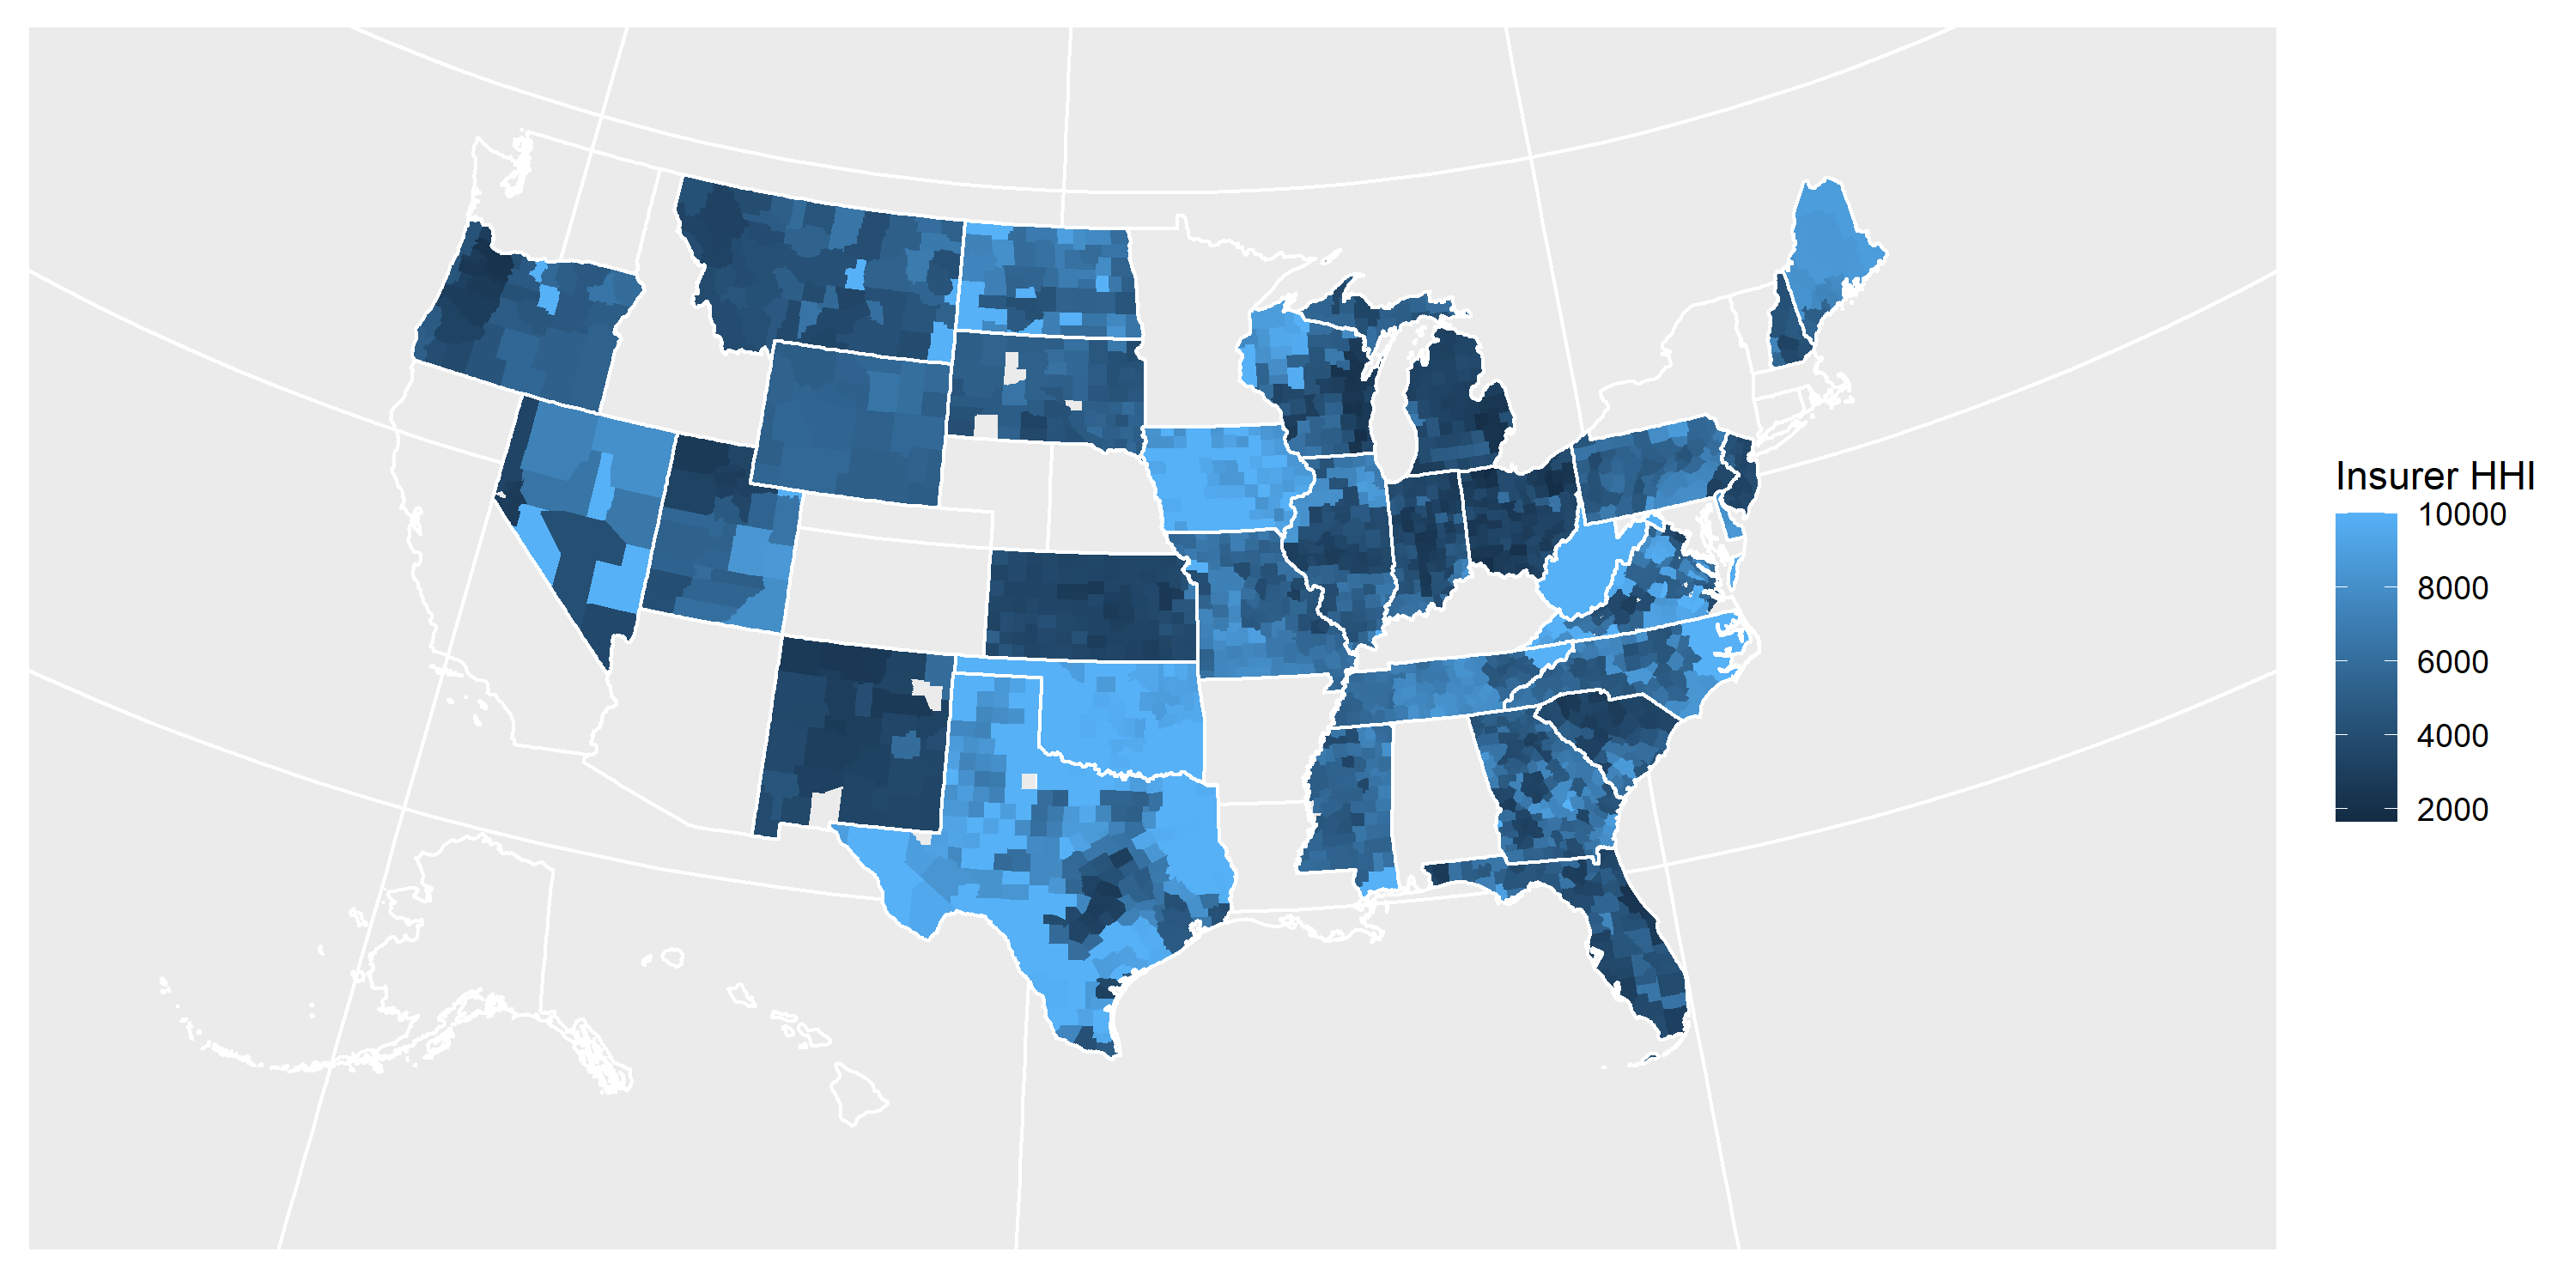
\includegraphics[height=3.5in,angle=0]{insurerHHI_2015.png}
\vspace{5mm}
\caption{Insurer HHI Heat Map, 2016}\label{Figure 6}
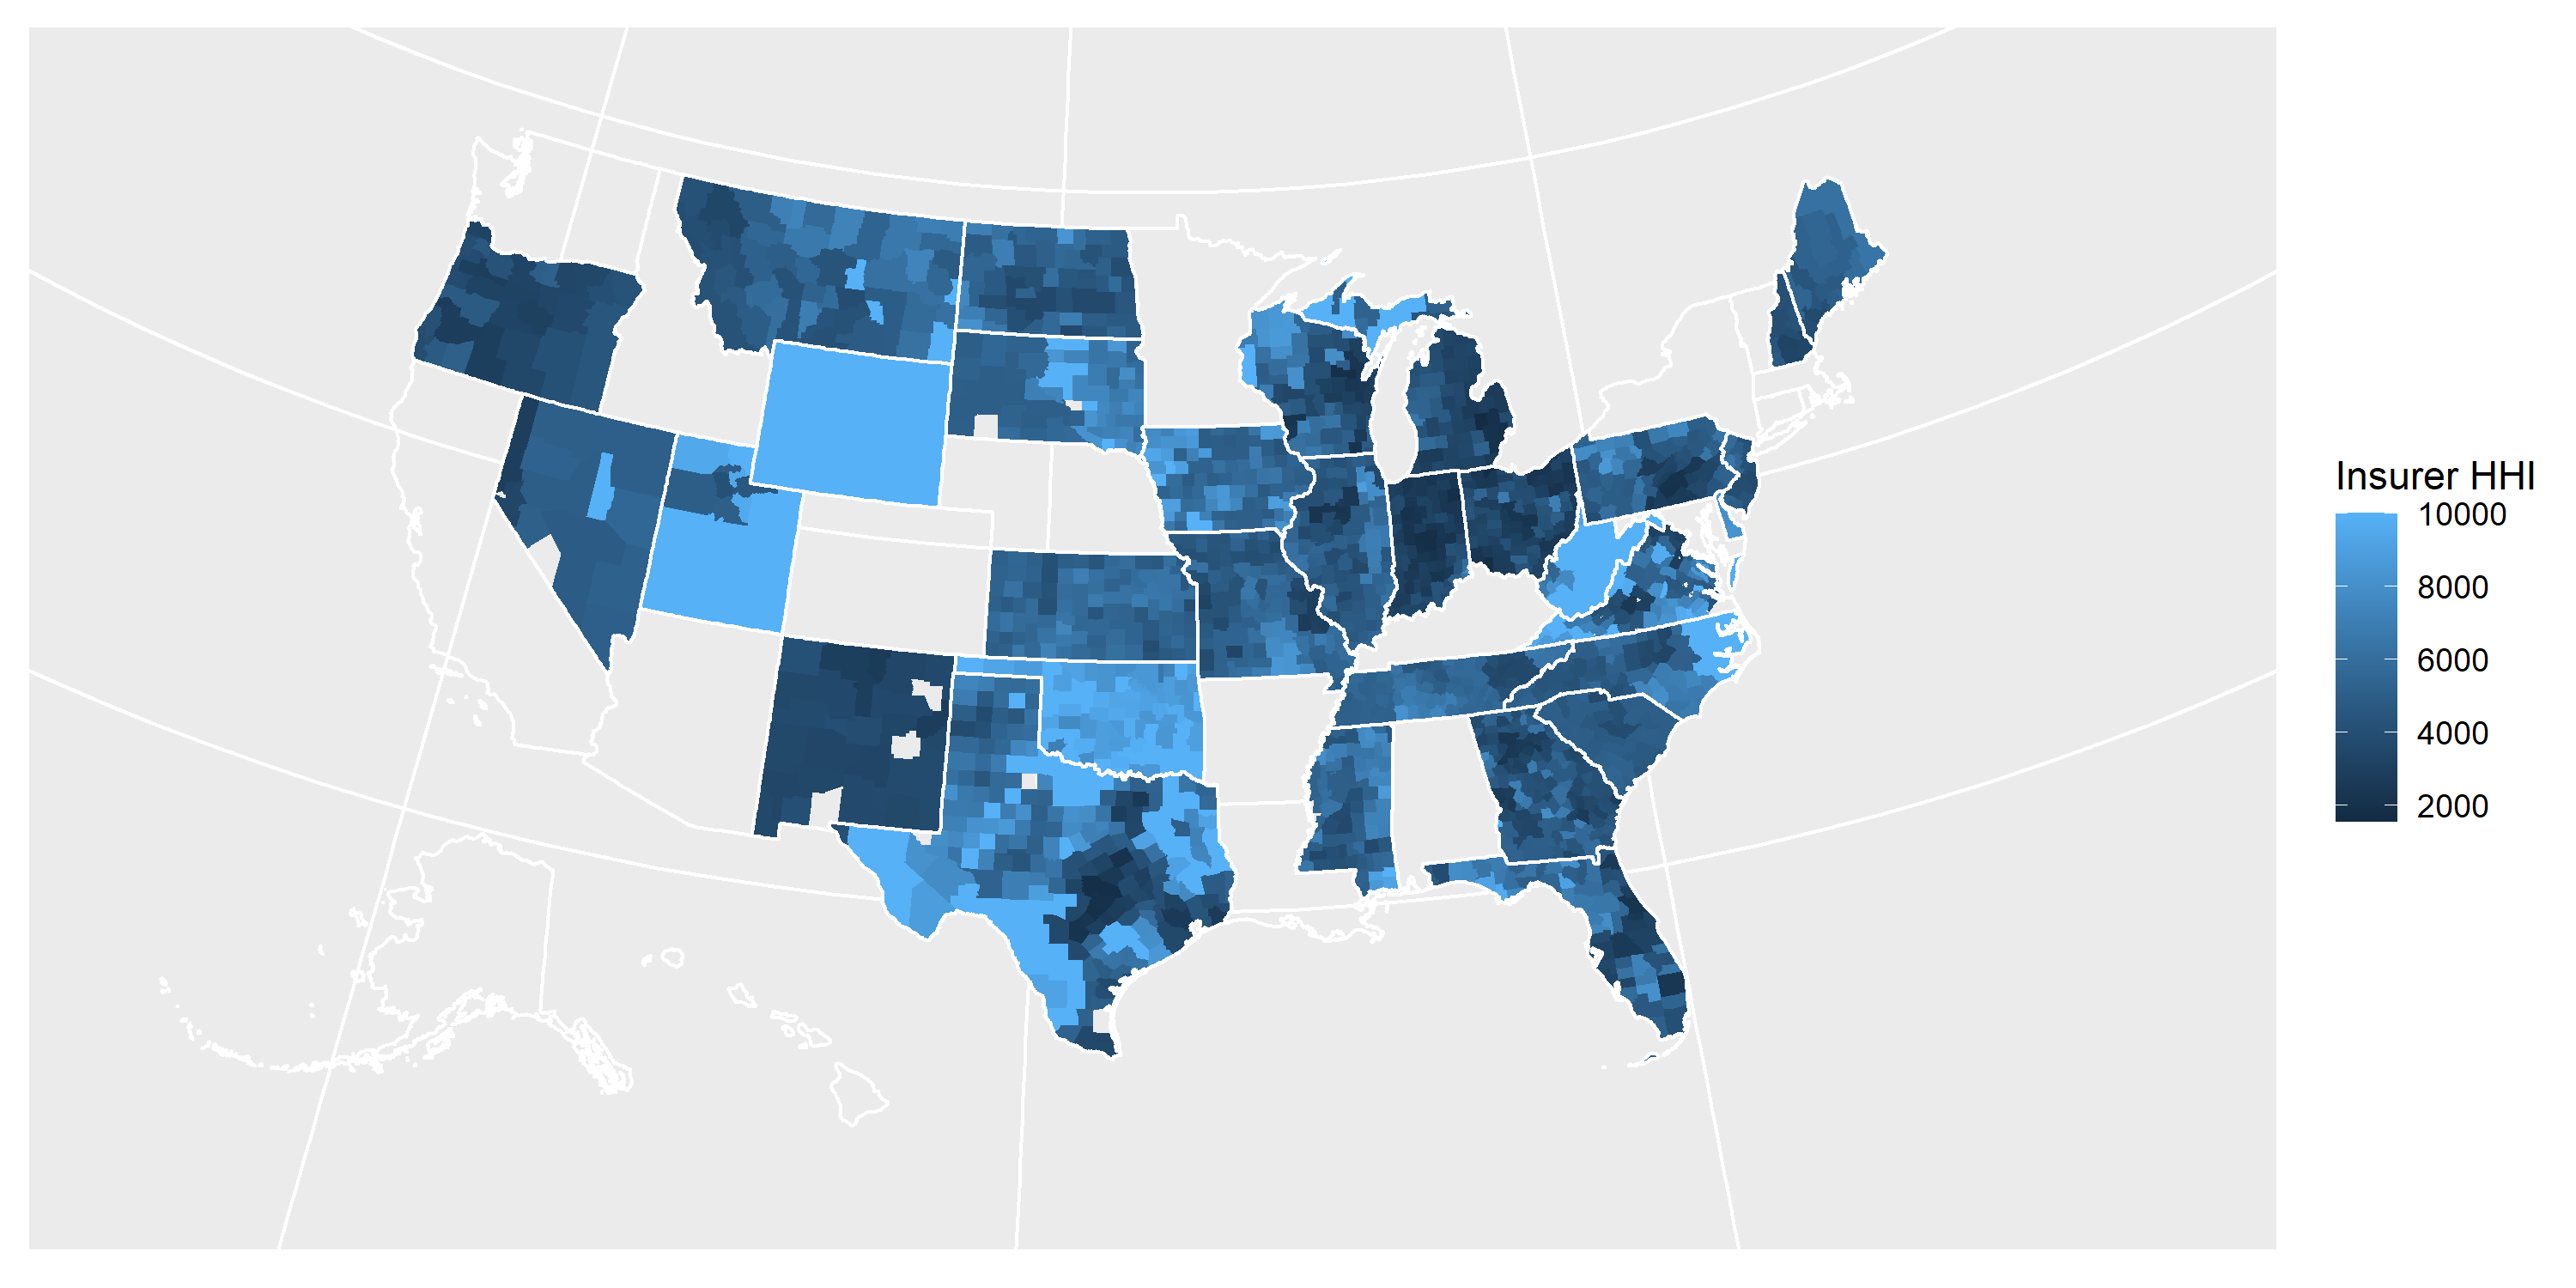
\includegraphics[height=3.5in,angle=0]{insurerHHI_2016.png}
\end{center}
\end{figure}

\begin{figure}[!h]
\begin{center}
\caption{Hospital HHI Heat Map, 2014}\label{Figure 7}
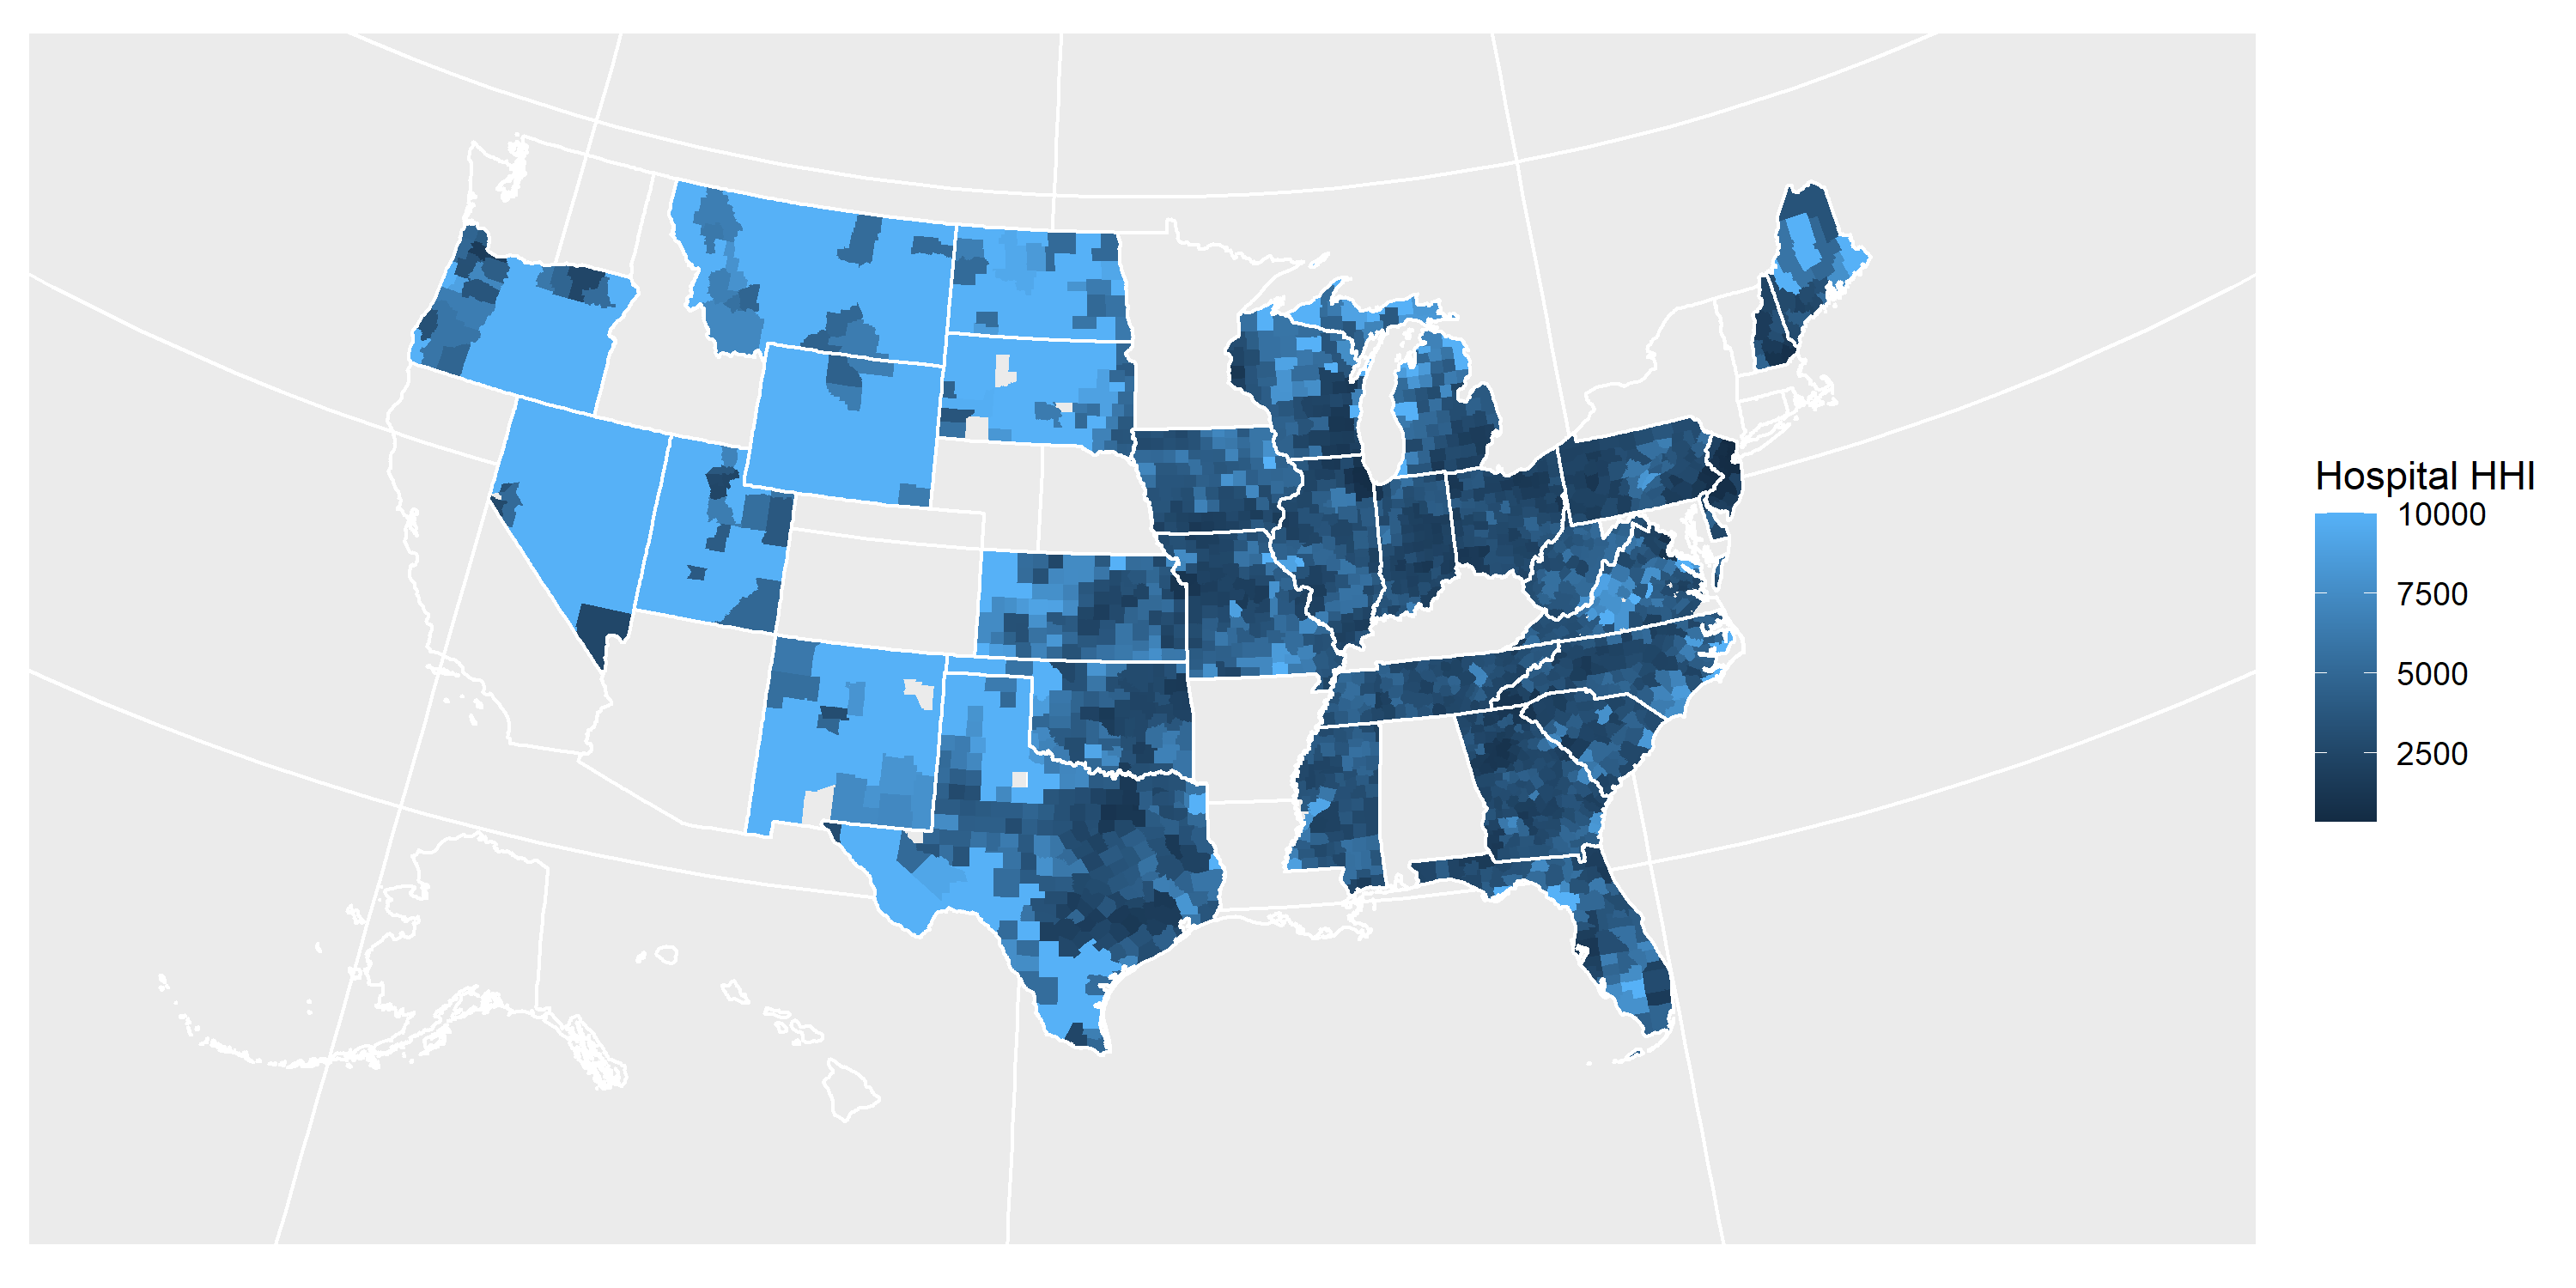
\includegraphics[height=3.5in,angle=0]{hospitalHHI_2014.png}
\vspace{5mm}
\caption{Hospital HHI Heat Map, 2015}\label{Figure 8}
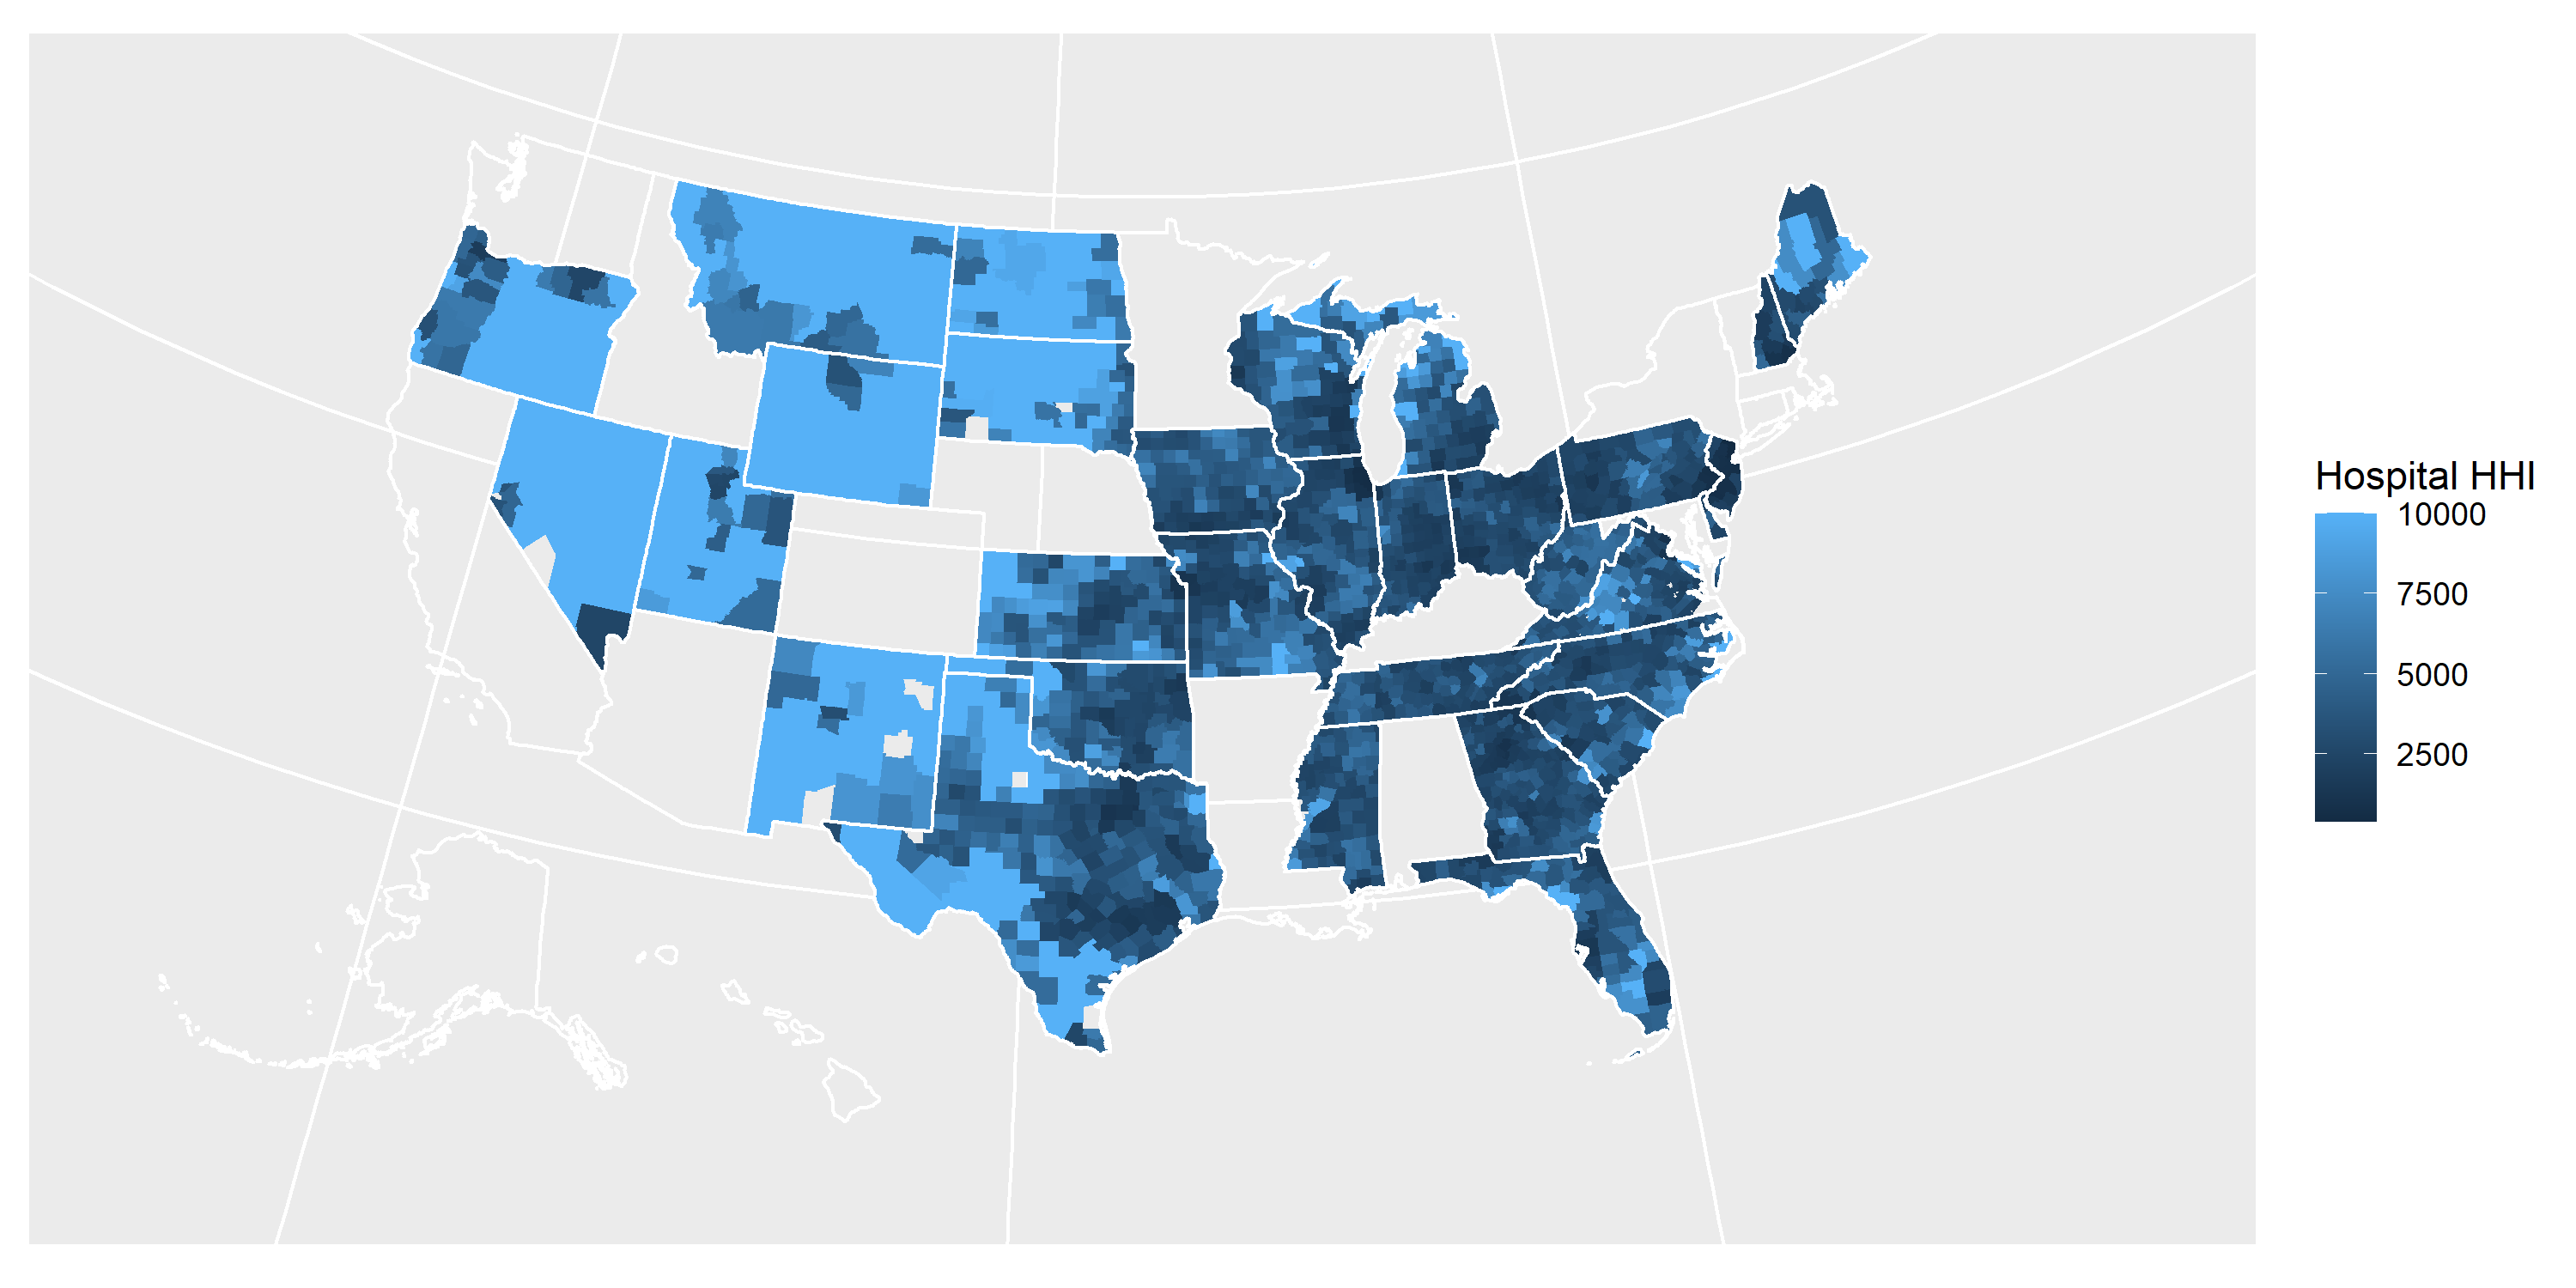
\includegraphics[height=3.5in,angle=0]{hospitalHHI_2015.png}
\end{center}
\end{figure}

\begin{figure}[!h]
\begin{center}
\caption{Regions Map}
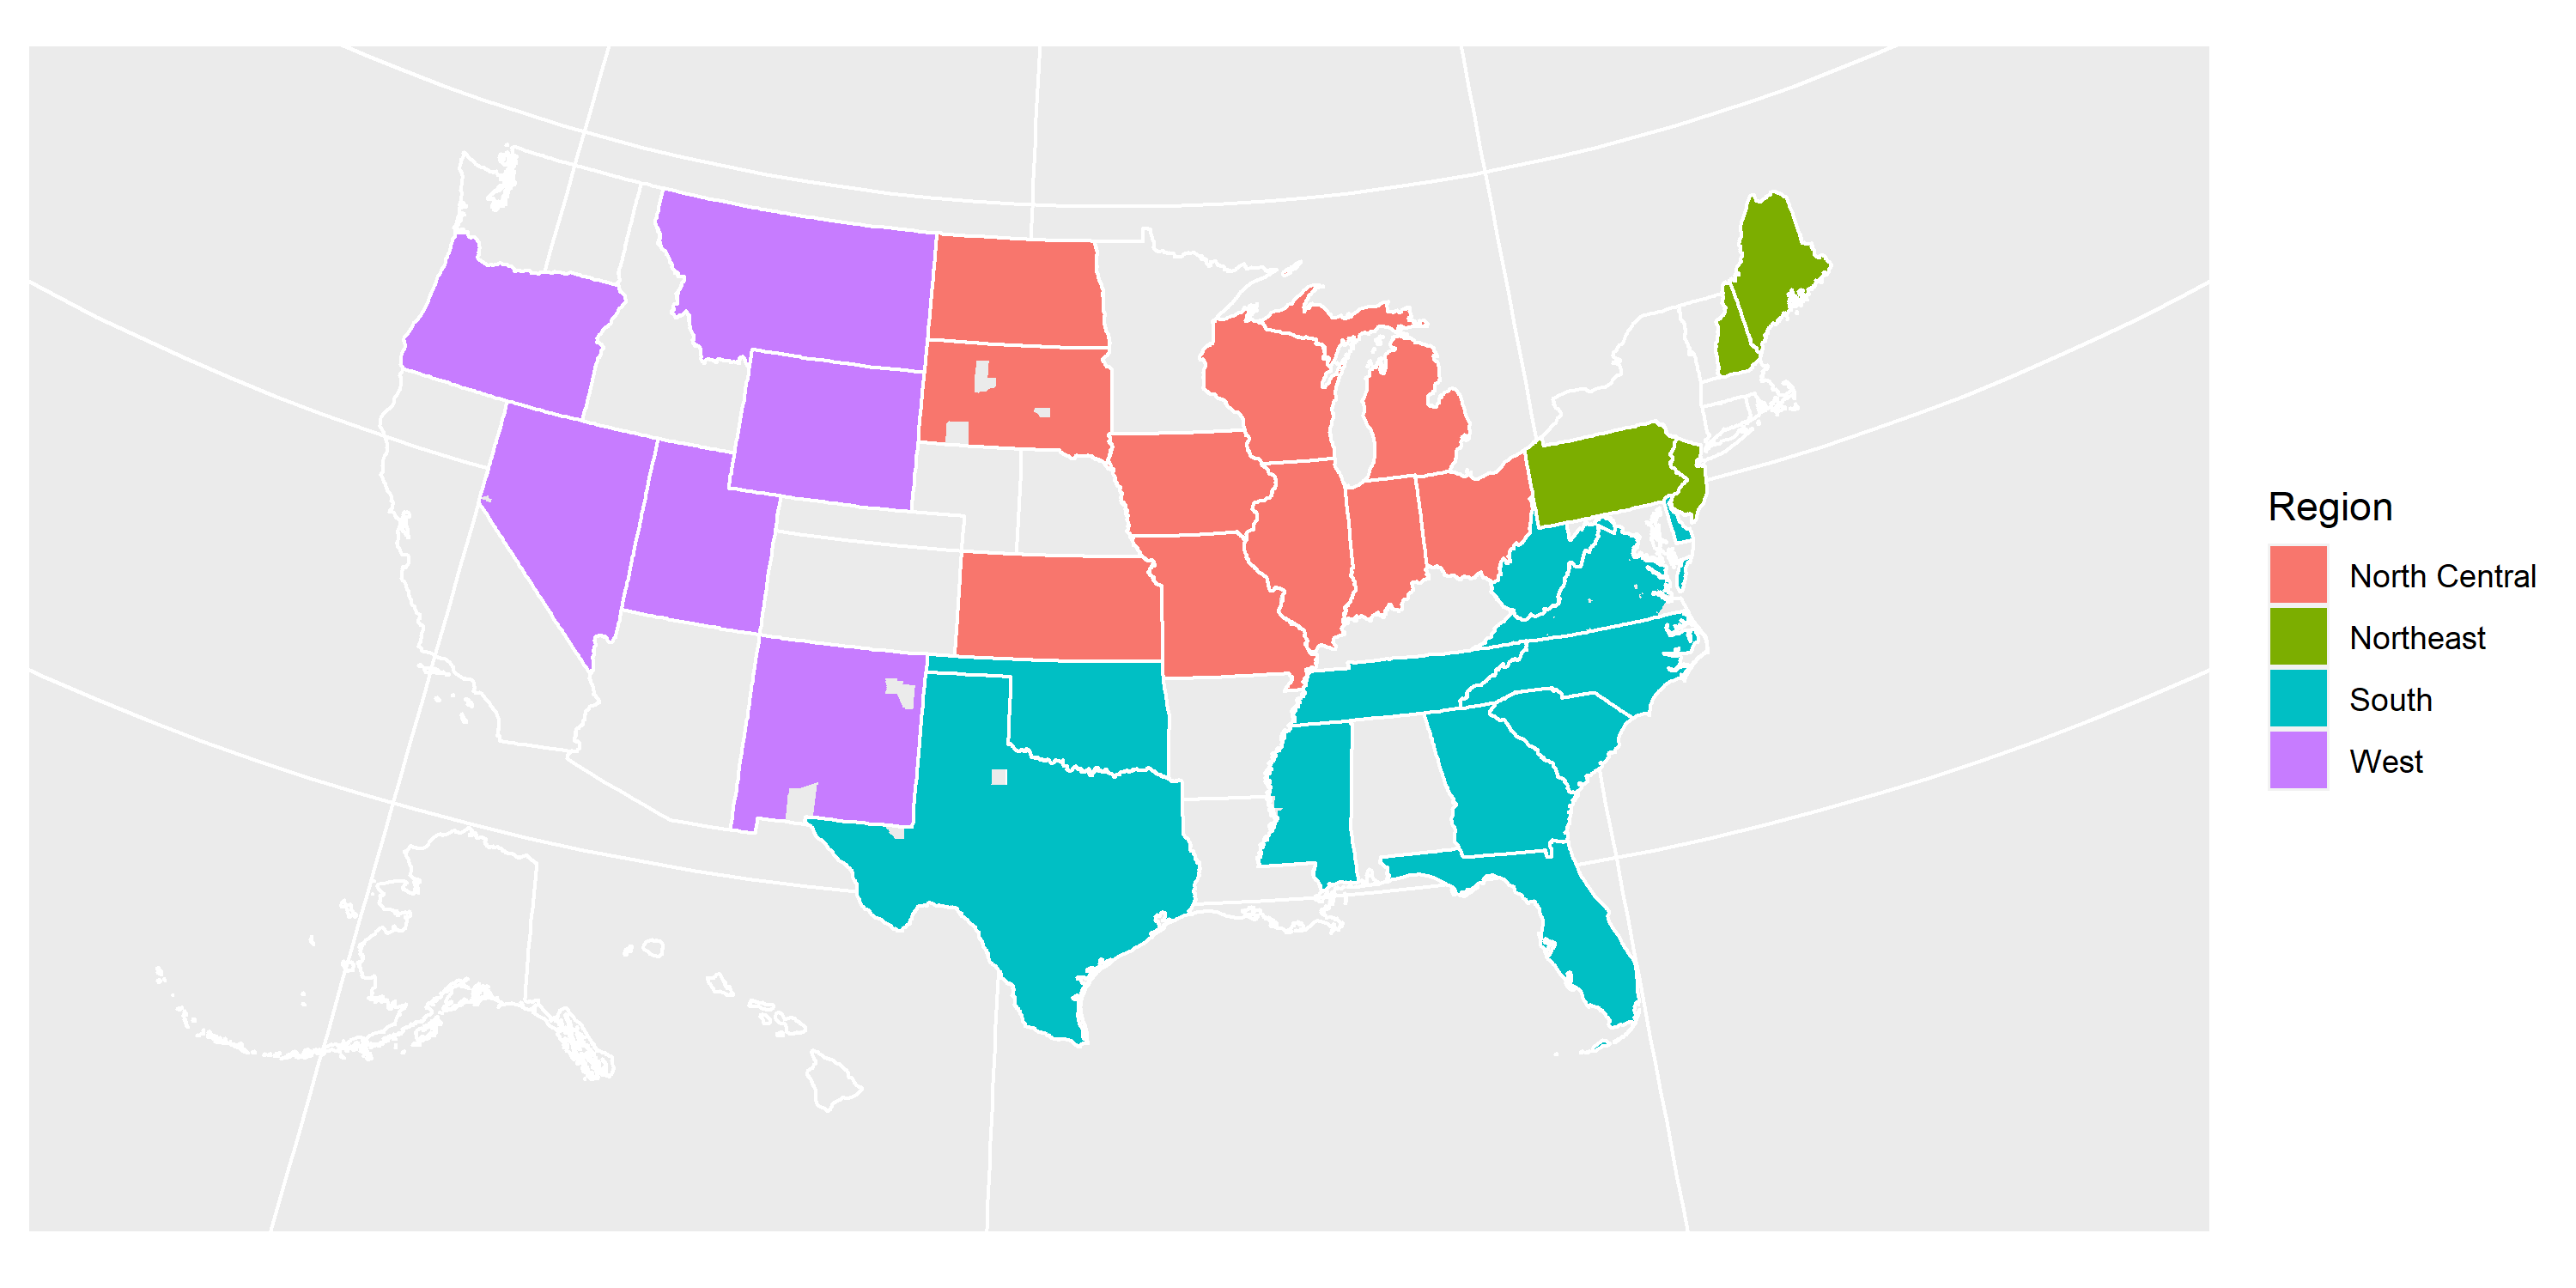
\includegraphics[height=3.5in,angle=0]{counties.png}
\end{center}
\end{figure}

\restoregeometry

\subsection{Alternative specifications}
As a robustness check, I fit several alternative specifications of my main model. I refit my main model using radii one standard deviation higher and lower than the values used in the paper (see Tables A.1 and A.2), and using radii estimated using only short-term general hospitals (see Table A.3). I add interaction terms for rurality and region to my main model (see Table A.4). I also modify my main model to use number of firms instead of logged HHI (see Table A.5; as in my HHI calculations, hospitals under the same health system are considered one firm). Tables summarizing these results, along with figures representing the bivariate relationship between logged insurer HHI and logged hospital HHI, can be found below.   

\vspace{2cm}

\begin{table}[!hb]
\centering
\caption{Main results (hospital market radius one SD lower)}

% Table created by stargazer v.5.2.2 by Marek Hlavac, Harvard University. E-mail: hlavac at fas.harvard.edu
% Date and time: Mon, Mar 15, 2021 - 11:56:58 PM
\begingroup 
\scriptsize 
\begin{tabular}{@{\extracolsep{5pt}}lccc} 
\\[-1.8ex]\hline 
\hline \\[-1.8ex] 
 & \multicolumn{3}{c}{\textit{Dependent variable:}} \\ 
\cline{2-4} 
\\[-1.8ex] & \multicolumn{3}{c}{Insurer HHI (logged)} \\ 
 & Main model & Boozary et al. (2019) & Griffith et al. (2018) \\ 
\\[-1.8ex] & (1) & (2) & (3)\\ 
\hline \\[-1.8ex] 
 Hospital HHI (logged) & 0.020$^{**}$ & 0.047$^{***}$ & 0.070$^{***}$ \\ 
  & (0.008) & (0.010) & (0.012) \\ 
  & & & \\ 
 No hospitals in market & 0.010 & 0.015 & 0.010 \\ 
  & (0.010) & (0.013) & (0.017) \\ 
  & & & \\ 
 Rurality (RUCC code) & 0.013$^{***}$ & 0.033$^{***}$ & 0.040$^{***}$ \\ 
  & (0.002) & (0.002) & (0.002) \\ 
  & & & \\ 
 Year &  &  & $-$0.073$^{***}$ \\ 
  &  &  & (0.011) \\ 
  & & & \\ 
\hline \\[-1.8ex] 
Observations & 4,128 & 4,410 & 4,410 \\ 
R$^{2}$ & 0.824 & 0.580 & 0.214 \\ 
Adjusted R$^{2}$ & 0.802 & 0.574 & 0.212 \\ 
Residual Std. Error & 0.182 (df = 3665) & 0.266 (df = 4339) & 0.362 (df = 4395) \\ 
F Statistic & 37.200$^{***}$ (df = 462; 3665) & 85.766$^{***}$ (df = 70; 4339) & 85.686$^{***}$ (df = 14; 4395) \\ 
\hline 
\hline \\[-1.8ex] 
\textit{Note:}  & \multicolumn{3}{r}{$^{*}$p$<$0.1; $^{**}$p$<$0.05; $^{***}$p$<$0.01} \\ 
 & \multicolumn{3}{r}{Controlling for rating area-year fixed effects in (1) and state-year fixed effects in (2).} \\ 
 & \multicolumn{3}{r}{Controlling for county/state covariates where appropriate.} \\ 
\end{tabular} 
\endgroup 

\end{table}

\begin{table}
\centering
\caption{Main results (hospital market radius one SD higher)}

% Table created by stargazer v.5.2.2 by Marek Hlavac, Harvard University. E-mail: hlavac at fas.harvard.edu
% Date and time: Mon, Mar 15, 2021 - 11:56:59 PM
\begingroup 
\scriptsize 
\begin{tabular}{@{\extracolsep{5pt}}lccc} 
\\[-1.8ex]\hline 
\hline \\[-1.8ex] 
 & \multicolumn{3}{c}{\textit{Dependent variable:}} \\ 
\cline{2-4} 
\\[-1.8ex] & \multicolumn{3}{c}{Insurer HHI (logged)} \\ 
 & Main model & Boozary et al. (2019) & Griffith et al. (2018) \\ 
\\[-1.8ex] & (1) & (2) & (3)\\ 
\hline \\[-1.8ex] 
 Hospital HHI (logged) & 0.027$^{***}$ & 0.023$^{**}$ & 0.034$^{***}$ \\ 
  & (0.008) & (0.009) & (0.010) \\ 
  & & & \\ 
 No hospitals in market & 0.016 & 0.022 & 0.014 \\ 
  & (0.022) & (0.031) & (0.041) \\ 
  & & & \\ 
 Rurality (RUCC code) & 0.013$^{***}$ & 0.035$^{***}$ & 0.042$^{***}$ \\ 
  & (0.002) & (0.002) & (0.002) \\ 
  & & & \\ 
 Year &  &  & $-$0.073$^{***}$ \\ 
  &  &  & (0.011) \\ 
  & & & \\ 
\hline \\[-1.8ex] 
Observations & 4,128 & 4,410 & 4,410 \\ 
R$^{2}$ & 0.824 & 0.578 & 0.210 \\ 
Adjusted R$^{2}$ & 0.802 & 0.572 & 0.207 \\ 
Residual Std. Error & 0.182 (df = 3665) & 0.267 (df = 4339) & 0.363 (df = 4395) \\ 
F Statistic & 37.245$^{***}$ (df = 462; 3665) & 85.034$^{***}$ (df = 70; 4339) & 83.353$^{***}$ (df = 14; 4395) \\ 
\hline 
\hline \\[-1.8ex] 
\textit{Note:}  & \multicolumn{3}{r}{$^{*}$p$<$0.1; $^{**}$p$<$0.05; $^{***}$p$<$0.01} \\ 
 & \multicolumn{3}{r}{Controlling for rating area-year fixed effects in (1) and state-year fixed effects in (2).} \\ 
 & \multicolumn{3}{r}{Controlling for county/state covariates where appropriate.} \\ 
\end{tabular} 
\endgroup 

\end{table}

\begin{table}
\centering
\caption{Main results (short-term general hospital market radius)}

% Table created by stargazer v.5.2.2 by Marek Hlavac, Harvard University. E-mail: hlavac at fas.harvard.edu
% Date and time: Mon, Mar 15, 2021 - 11:57:00 PM
\begingroup 
\scriptsize 
\begin{tabular}{@{\extracolsep{5pt}}lccc} 
\\[-1.8ex]\hline 
\hline \\[-1.8ex] 
 & \multicolumn{3}{c}{\textit{Dependent variable:}} \\ 
\cline{2-4} 
\\[-1.8ex] & \multicolumn{3}{c}{Insurer HHI (logged)} \\ 
 & Main model & Boozary et al. (2019) & Griffith et al. (2018) \\ 
\\[-1.8ex] & (1) & (2) & (3)\\ 
\hline \\[-1.8ex] 
 Hospital HHI (logged) & 0.035$^{***}$ & 0.063$^{***}$ & 0.090$^{***}$ \\ 
  & (0.008) & (0.010) & (0.012) \\ 
  & & & \\ 
 No hospitals in market & 0.014 & 0.013 & $-$0.004 \\ 
  & (0.010) & (0.013) & (0.016) \\ 
  & & & \\ 
 Rurality (RUCC code) & 0.012$^{***}$ & 0.031$^{***}$ & 0.037$^{***}$ \\ 
  & (0.002) & (0.002) & (0.003) \\ 
  & & & \\ 
 Year &  &  & $-$0.074$^{***}$ \\ 
  &  &  & (0.011) \\ 
  & & & \\ 
\hline \\[-1.8ex] 
Observations & 4,128 & 4,410 & 4,410 \\ 
R$^{2}$ & 0.825 & 0.582 & 0.218 \\ 
Adjusted R$^{2}$ & 0.803 & 0.575 & 0.215 \\ 
Residual Std. Error & 0.182 (df = 3665) & 0.266 (df = 4339) & 0.361 (df = 4395) \\ 
F Statistic & 37.379$^{***}$ (df = 462; 3665) & 86.382$^{***}$ (df = 70; 4339) & 87.452$^{***}$ (df = 14; 4395) \\ 
\hline 
\hline \\[-1.8ex] 
\textit{Note:}  & \multicolumn{3}{r}{$^{*}$p$<$0.1; $^{**}$p$<$0.05; $^{***}$p$<$0.01} \\ 
 & \multicolumn{3}{r}{Controlling for rating area-year fixed effects in (1) and state-year fixed effects in (2).} \\ 
 & \multicolumn{3}{r}{Controlling for county/state covariates where appropriate.} \\ 
\end{tabular} 
\endgroup 

\end{table}

\newgeometry{left=1cm, right=1cm, bottom=1.9cm}
\begin{table}
\centering
\caption{Main results (with interaction terms)}

% Table created by stargazer v.5.2.2 by Marek Hlavac, Harvard University. E-mail: hlavac at fas.harvard.edu
% Date and time: Mon, Mar 15, 2021 - 11:57:02 PM
\begingroup 
\scriptsize 
\begin{tabular}{@{\extracolsep{5pt}}lcc} 
\\[-1.8ex]\hline 
\hline \\[-1.8ex] 
 & \multicolumn{2}{c}{\textit{Dependent variable:}} \\ 
\cline{2-3} 
\\[-1.8ex] & \multicolumn{2}{c}{Insurer HHI (logged)} \\ 
 & Rurality (RUCC code) interaction & Region interaction \\ 
\\[-1.8ex] & (1) & (2)\\ 
\hline \\[-1.8ex] 
 Hospital HHI (logged) & 0.034$^{***}$ & 0.027$^{**}$ \\ 
  & (0.008) & (0.013) \\ 
  & & \\ 
 No hospitals in market & 0.015 & 0.017 \\ 
  & (0.015) & (0.016) \\ 
  & & \\ 
 Hospital HHI (logged) * RUCC code 4-6 & $-$0.003 &  \\ 
  & (0.002) &  \\ 
  & & \\ 
 Hospital HHI (logged) * RUCC code 7-9 & $-$0.001 &  \\ 
  & (0.003) &  \\ 
  & & \\ 
 Hospital HHI (logged) * South &  & 0.011 \\ 
  &  & (0.031) \\ 
  & & \\ 
 Hospital HHI (logged) * North Central &  & 0.009 \\ 
  &  & (0.017) \\ 
  & & \\ 
 Hospital HHI (logged) * West &  & 0.020 \\ 
  &  & (0.035) \\ 
  & & \\ 
\hline \\[-1.8ex] 
Observations & 4,128 & 4,128 \\ 
R$^{2}$ & 0.825 & 0.825 \\ 
Adjusted R$^{2}$ & 0.803 & 0.803 \\ 
Residual Std. Error & 0.182 (df = 3663) & 0.182 (df = 3662) \\ 
F Statistic & 37.262$^{***}$ (df = 464; 3663) & 37.088$^{***}$ (df = 465; 3662) \\ 
\hline 
\hline \\[-1.8ex] 
\textit{Note:}  & \multicolumn{2}{r}{$^{*}$p$<$0.1; $^{**}$p$<$0.05; $^{***}$p$<$0.01} \\ 
 & \multicolumn{2}{r}{Also controlling for rating area-year fixed effects, and county covariates.} \\ 
 & \multicolumn{2}{r}{Coefficient for Hospital HHI (logged) centered at RUCC codes 1-3 in (1), and Northeast region in (2)} \\ 
\end{tabular} 
\endgroup 

\end{table}
\restoregeometry

\begin{table}
\centering
\caption{Main results (number of firms)}

% Table created by stargazer v.5.2.2 by Marek Hlavac, Harvard University. E-mail: hlavac at fas.harvard.edu
% Date and time: Mon, Mar 15, 2021 - 11:56:55 PM
\begingroup 
\scriptsize 
\begin{tabular}{@{\extracolsep{5pt}}lccc} 
\\[-1.8ex]\hline 
\hline \\[-1.8ex] 
 & \multicolumn{3}{c}{\textit{Dependent variable:}} \\ 
\cline{2-4} 
\\[-1.8ex] & \multicolumn{3}{c}{Number of insurers} \\ 
 & Main model & Boozary et al. (2019) & Griffith et al. (2018) \\ 
\\[-1.8ex] & (1) & (2) & (3)\\ 
\hline \\[-1.8ex] 
 Number of hospitals & 0.019$^{***}$ & 0.028$^{***}$ & 0.025$^{***}$ \\ 
  & (0.002) & (0.003) & (0.003) \\ 
  & & & \\ 
 No hospitals in market & $-$0.035 & $-$0.096 & $-$0.383$^{***}$ \\ 
  & (0.058) & (0.083) & (0.109) \\ 
  & & & \\ 
 Rurality (RUCC code) & $-$0.066$^{***}$ & $-$0.152$^{***}$ & $-$0.221$^{***}$ \\ 
  & (0.007) & (0.008) & (0.010) \\ 
  & & & \\ 
 Year &  &  & $-$0.234$^{***}$ \\ 
  &  &  & (0.045) \\ 
  & & & \\ 
\hline \\[-1.8ex] 
Observations & 4,128 & 4,410 & 4,410 \\ 
R$^{2}$ & 0.872 & 0.675 & 0.335 \\ 
Adjusted R$^{2}$ & 0.855 & 0.670 & 0.333 \\ 
Residual Std. Error & 0.693 (df = 3665) & 1.040 (df = 4339) & 1.479 (df = 4395) \\ 
F Statistic & 53.824$^{***}$ (df = 462; 3665) & 128.810$^{***}$ (df = 70; 4339) & 158.066$^{***}$ (df = 14; 4395) \\ 
\hline 
\hline \\[-1.8ex] 
\textit{Note:}  & \multicolumn{3}{r}{$^{*}$p$<$0.1; $^{**}$p$<$0.05; $^{***}$p$<$0.01} \\ 
 & \multicolumn{3}{r}{Also controlling for rating area-year fixed effects and county covariates.} \\ 
\end{tabular} 
\endgroup 

\end{table}

\clearpage

\begin{figure}[!h]
\begin{center}
\caption{Logged insurer HHI vs. hospital HHI, scatterplot}
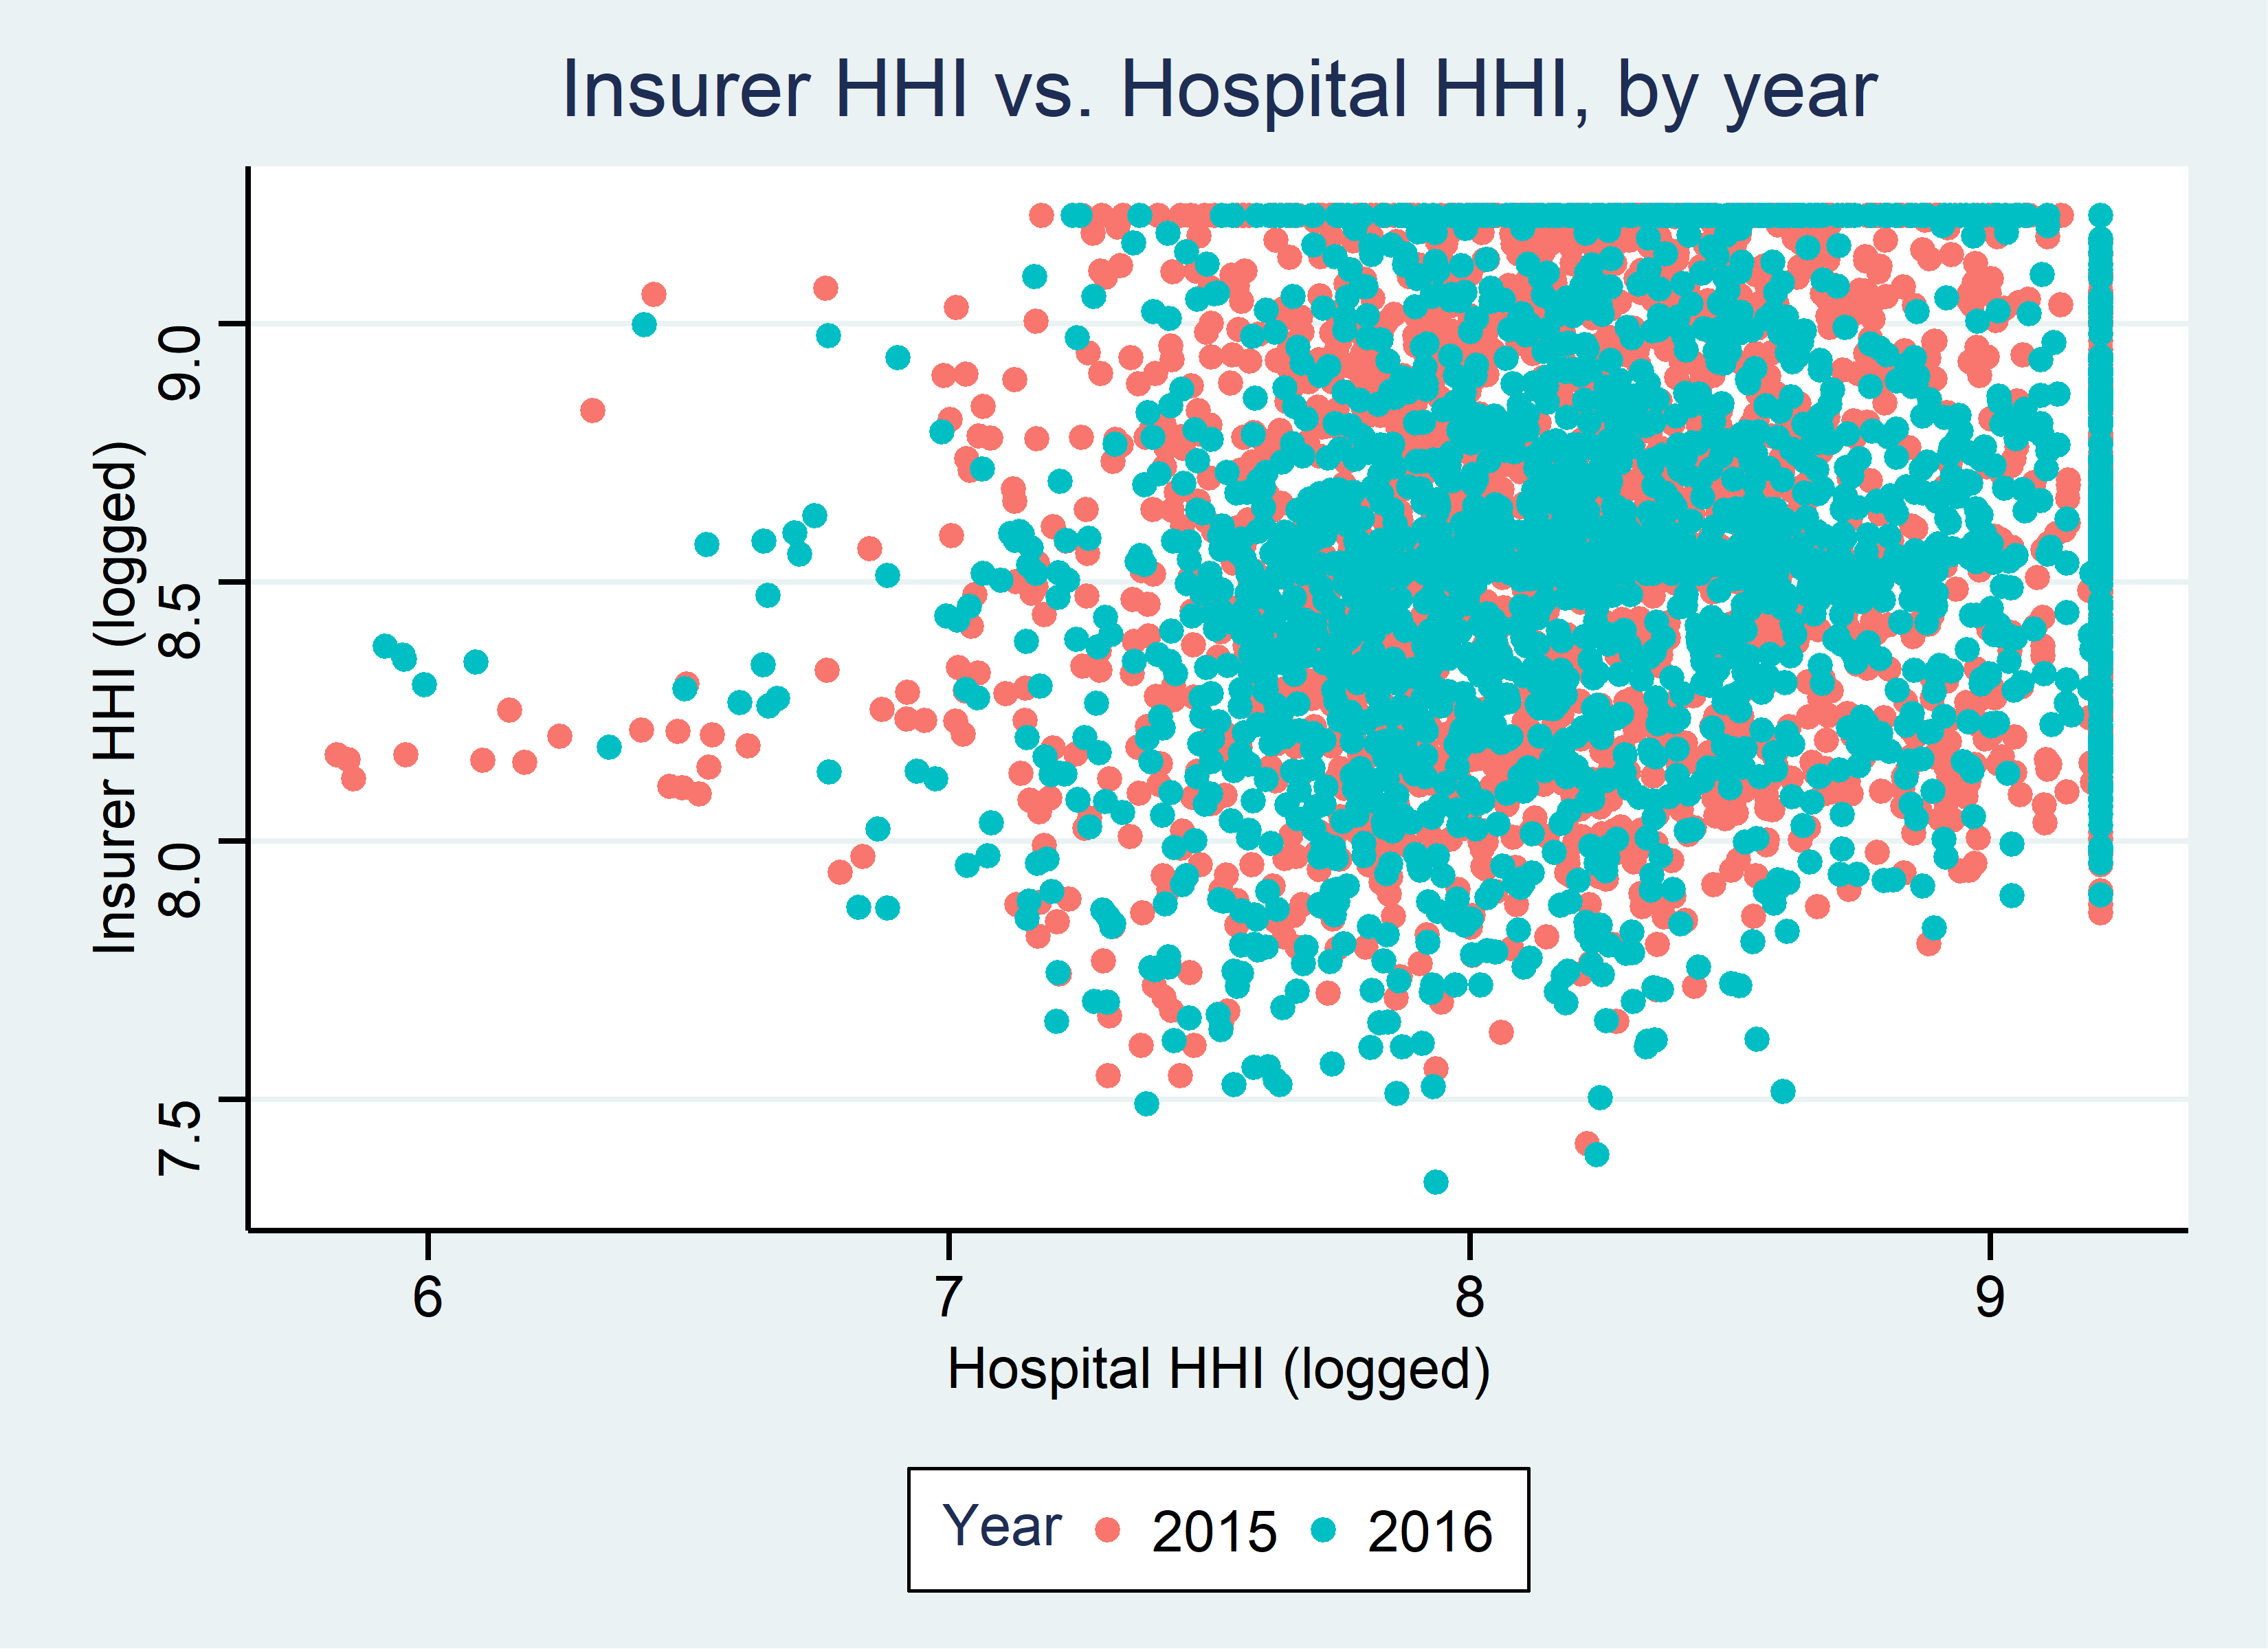
\includegraphics[height=3.5in,angle=0]{scatter_byyear.png}
\end{center}
\end{figure}

\begin{figure}[!h]
\begin{center}
\caption{Logged insurer HHI vs. hospital HHI, binned scatterplot}
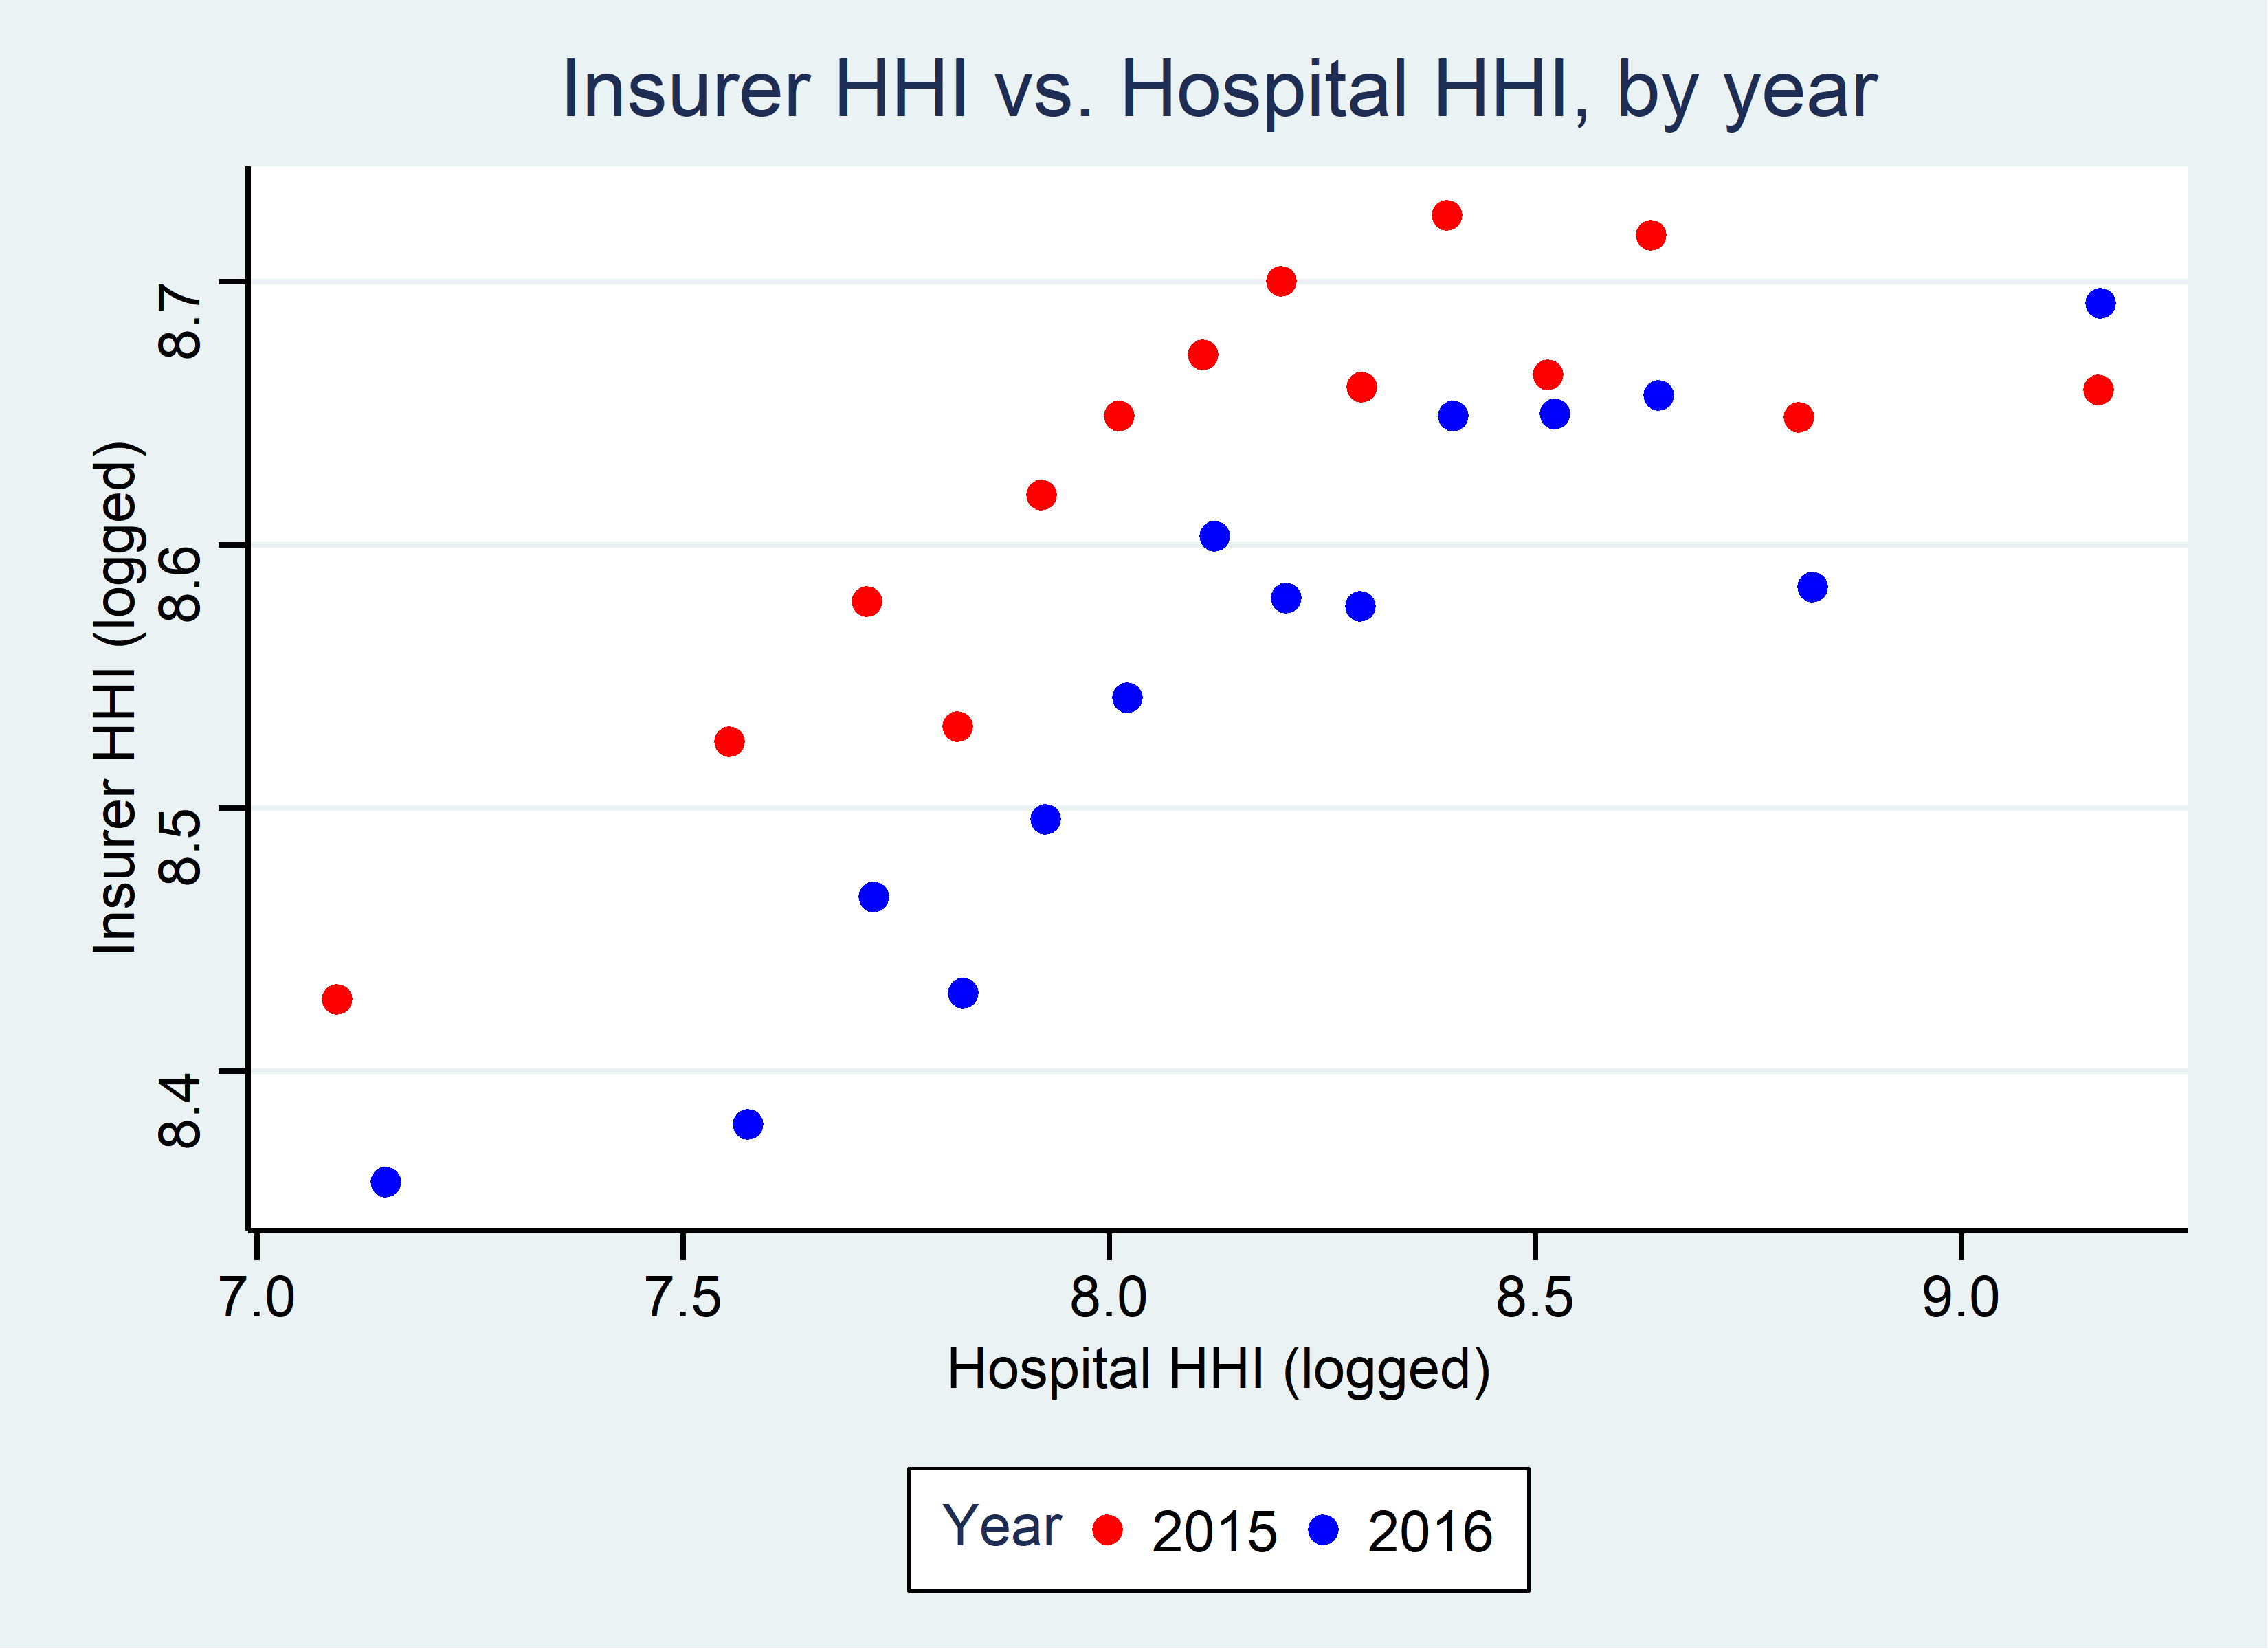
\includegraphics[height=3.5in,angle=0]{binnedscatter_byyear.png}
\end{center}
\end{figure}

\clearpage

\subsection{Non-normality of model residuals}
My main model's residuals fail the Shapiro-Wilk's test of normality, due seemingly to outlier values at the tails of my dependent variable distribution. This doesn't undermine the properties of my coefficient of interest estimate (i.e. OLS remains BLUE), but it does call into question my standard errors and p-values. Because I already log-linearize my dependent variable for interpretation purposes, winsorizing is an ineffective option. Instead, I bootstrap my regression, following the procedure outlined by \citet{fox_bootstrapping_2017}. The 99 percent confidence interval around my empirical distribution for my coefficient of interest is (.01, .06), which is about in line with what one would expect from my cluster-robust standard errors (i.e. I again reject the null hypothesis at significance $p<.01$). Graphs of my model residuals, as well as my bootstrapped coefficient distribution, can be found below.
\vspace{1cm}
\begin{figure}[!h]
\begin{center}
\caption{Histogram of residuals (main model)}
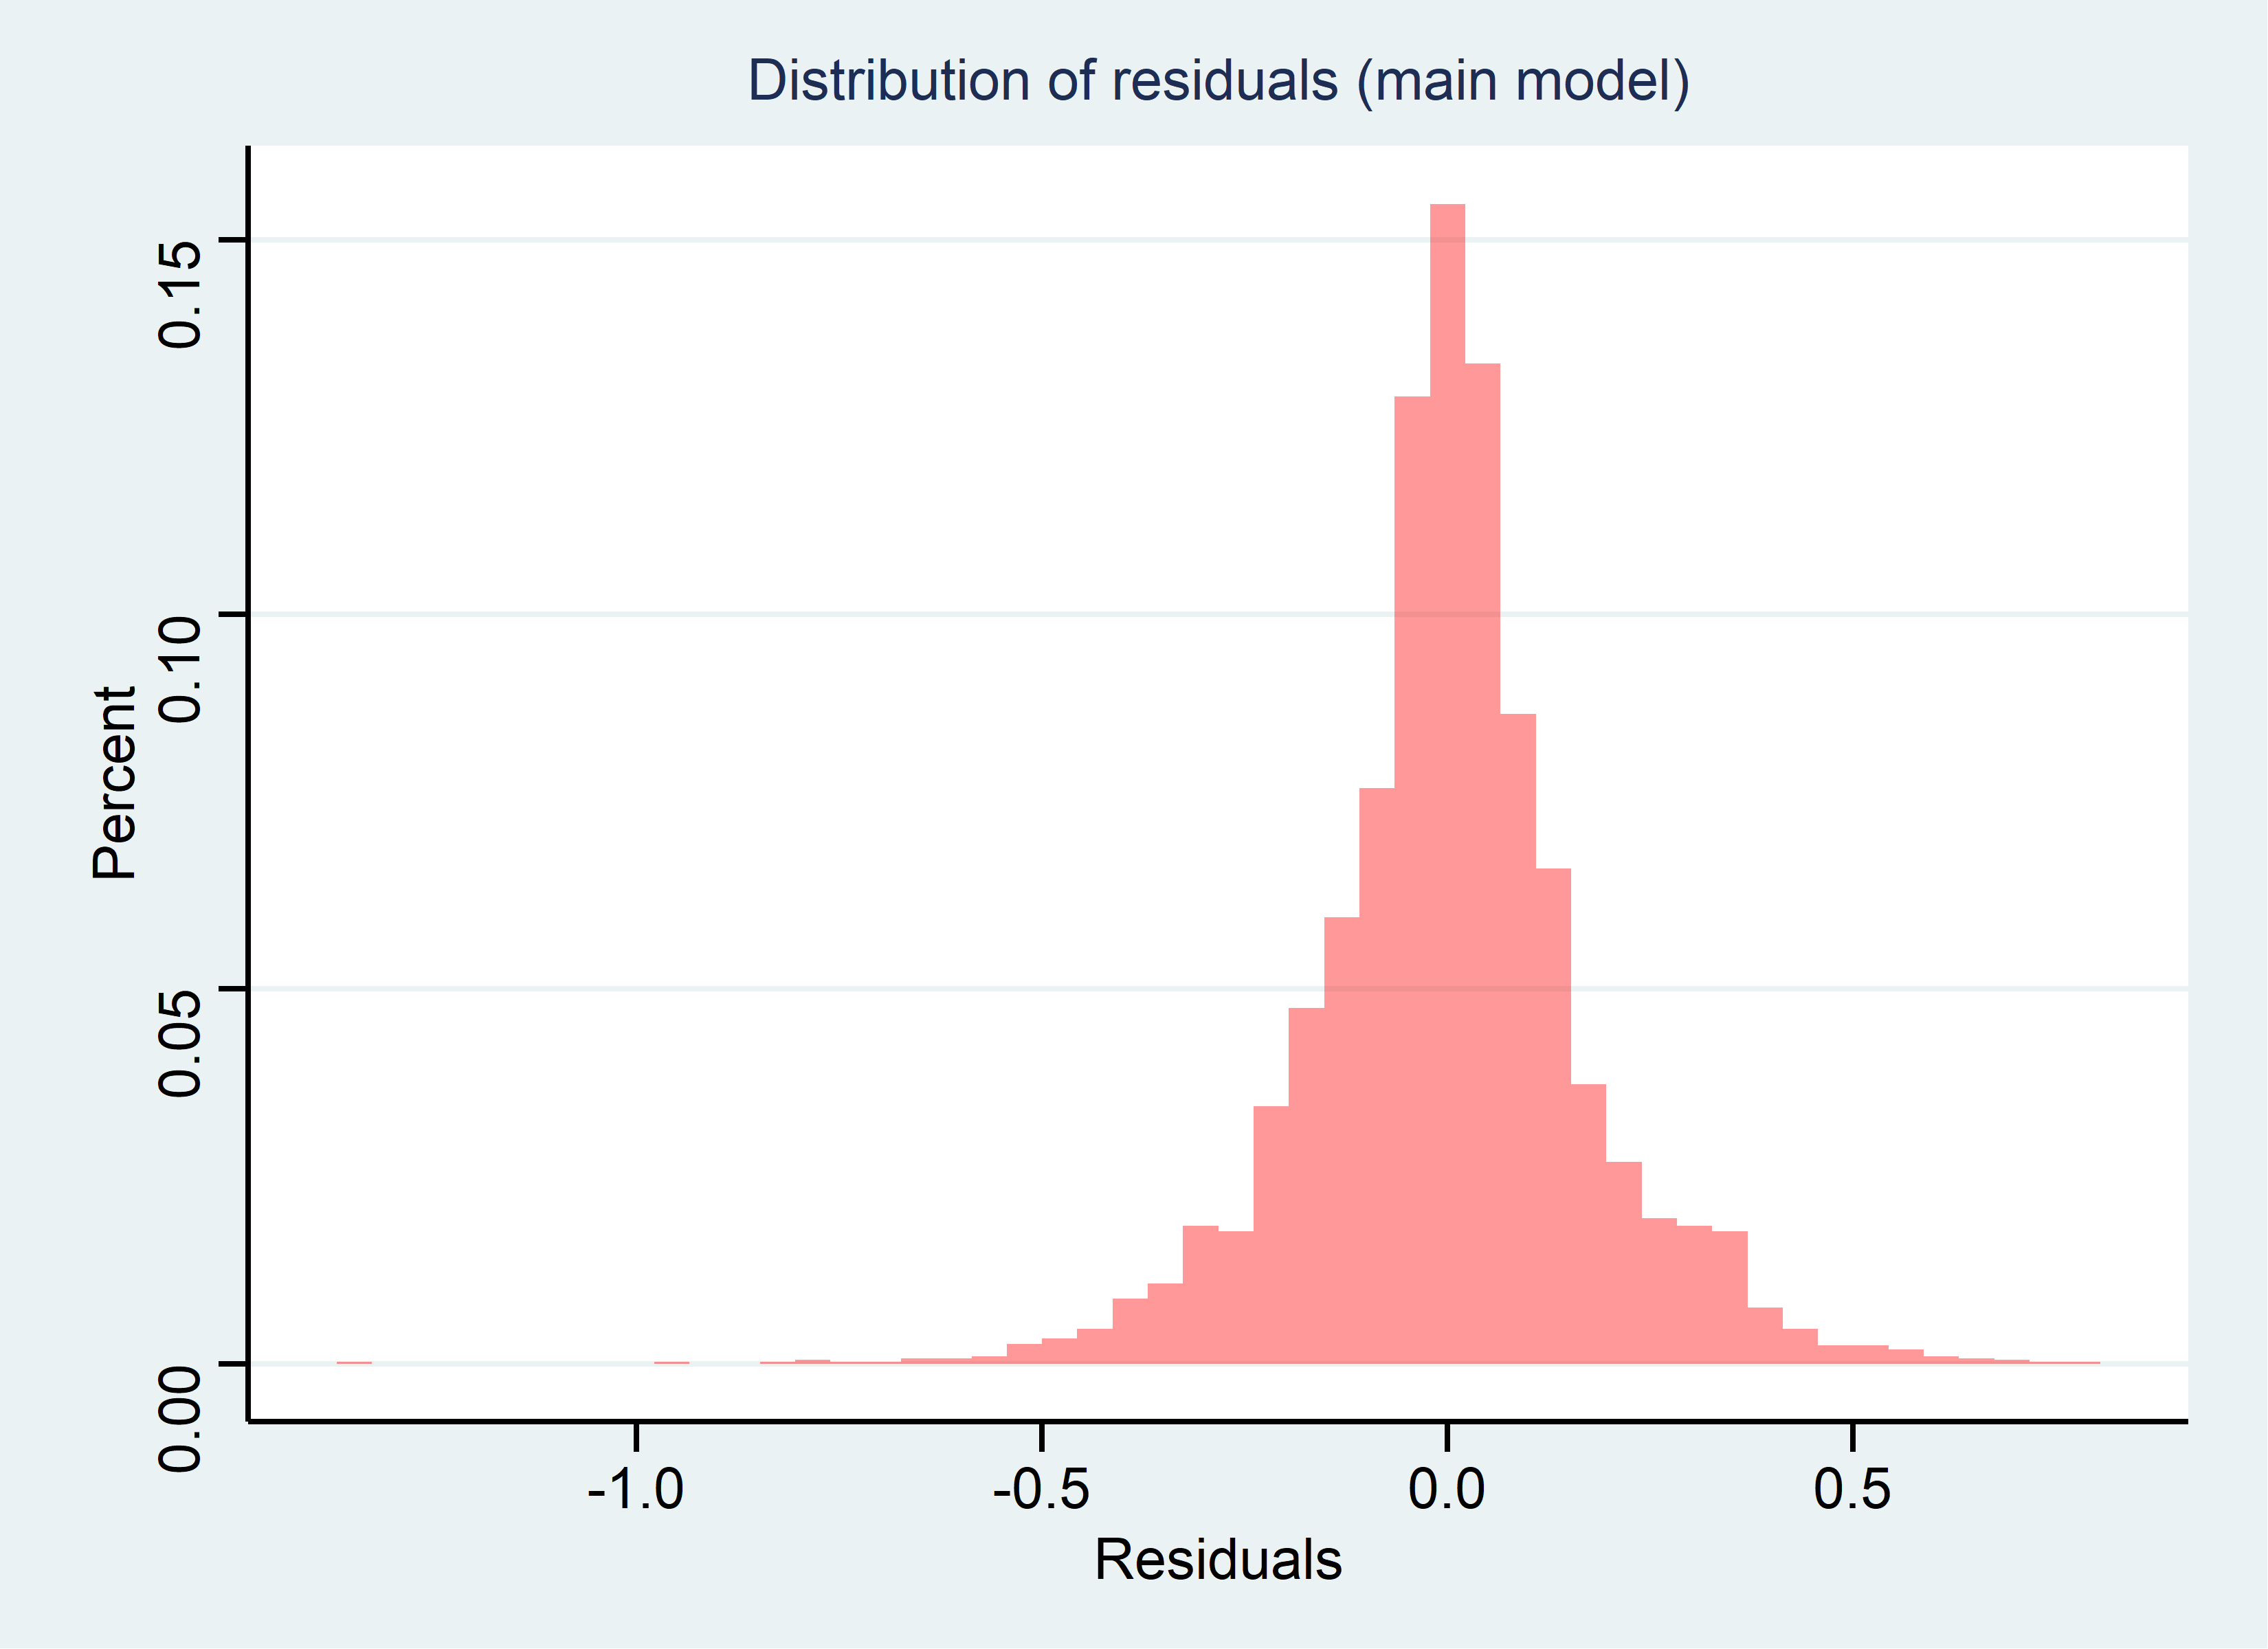
\includegraphics[height=4in,angle=0]{hist_resid_mainmodel.png}
\end{center}
\end{figure}
\begin{figure}[!h]
\begin{center}
\caption{Q-Q plot of residuals (main model)}
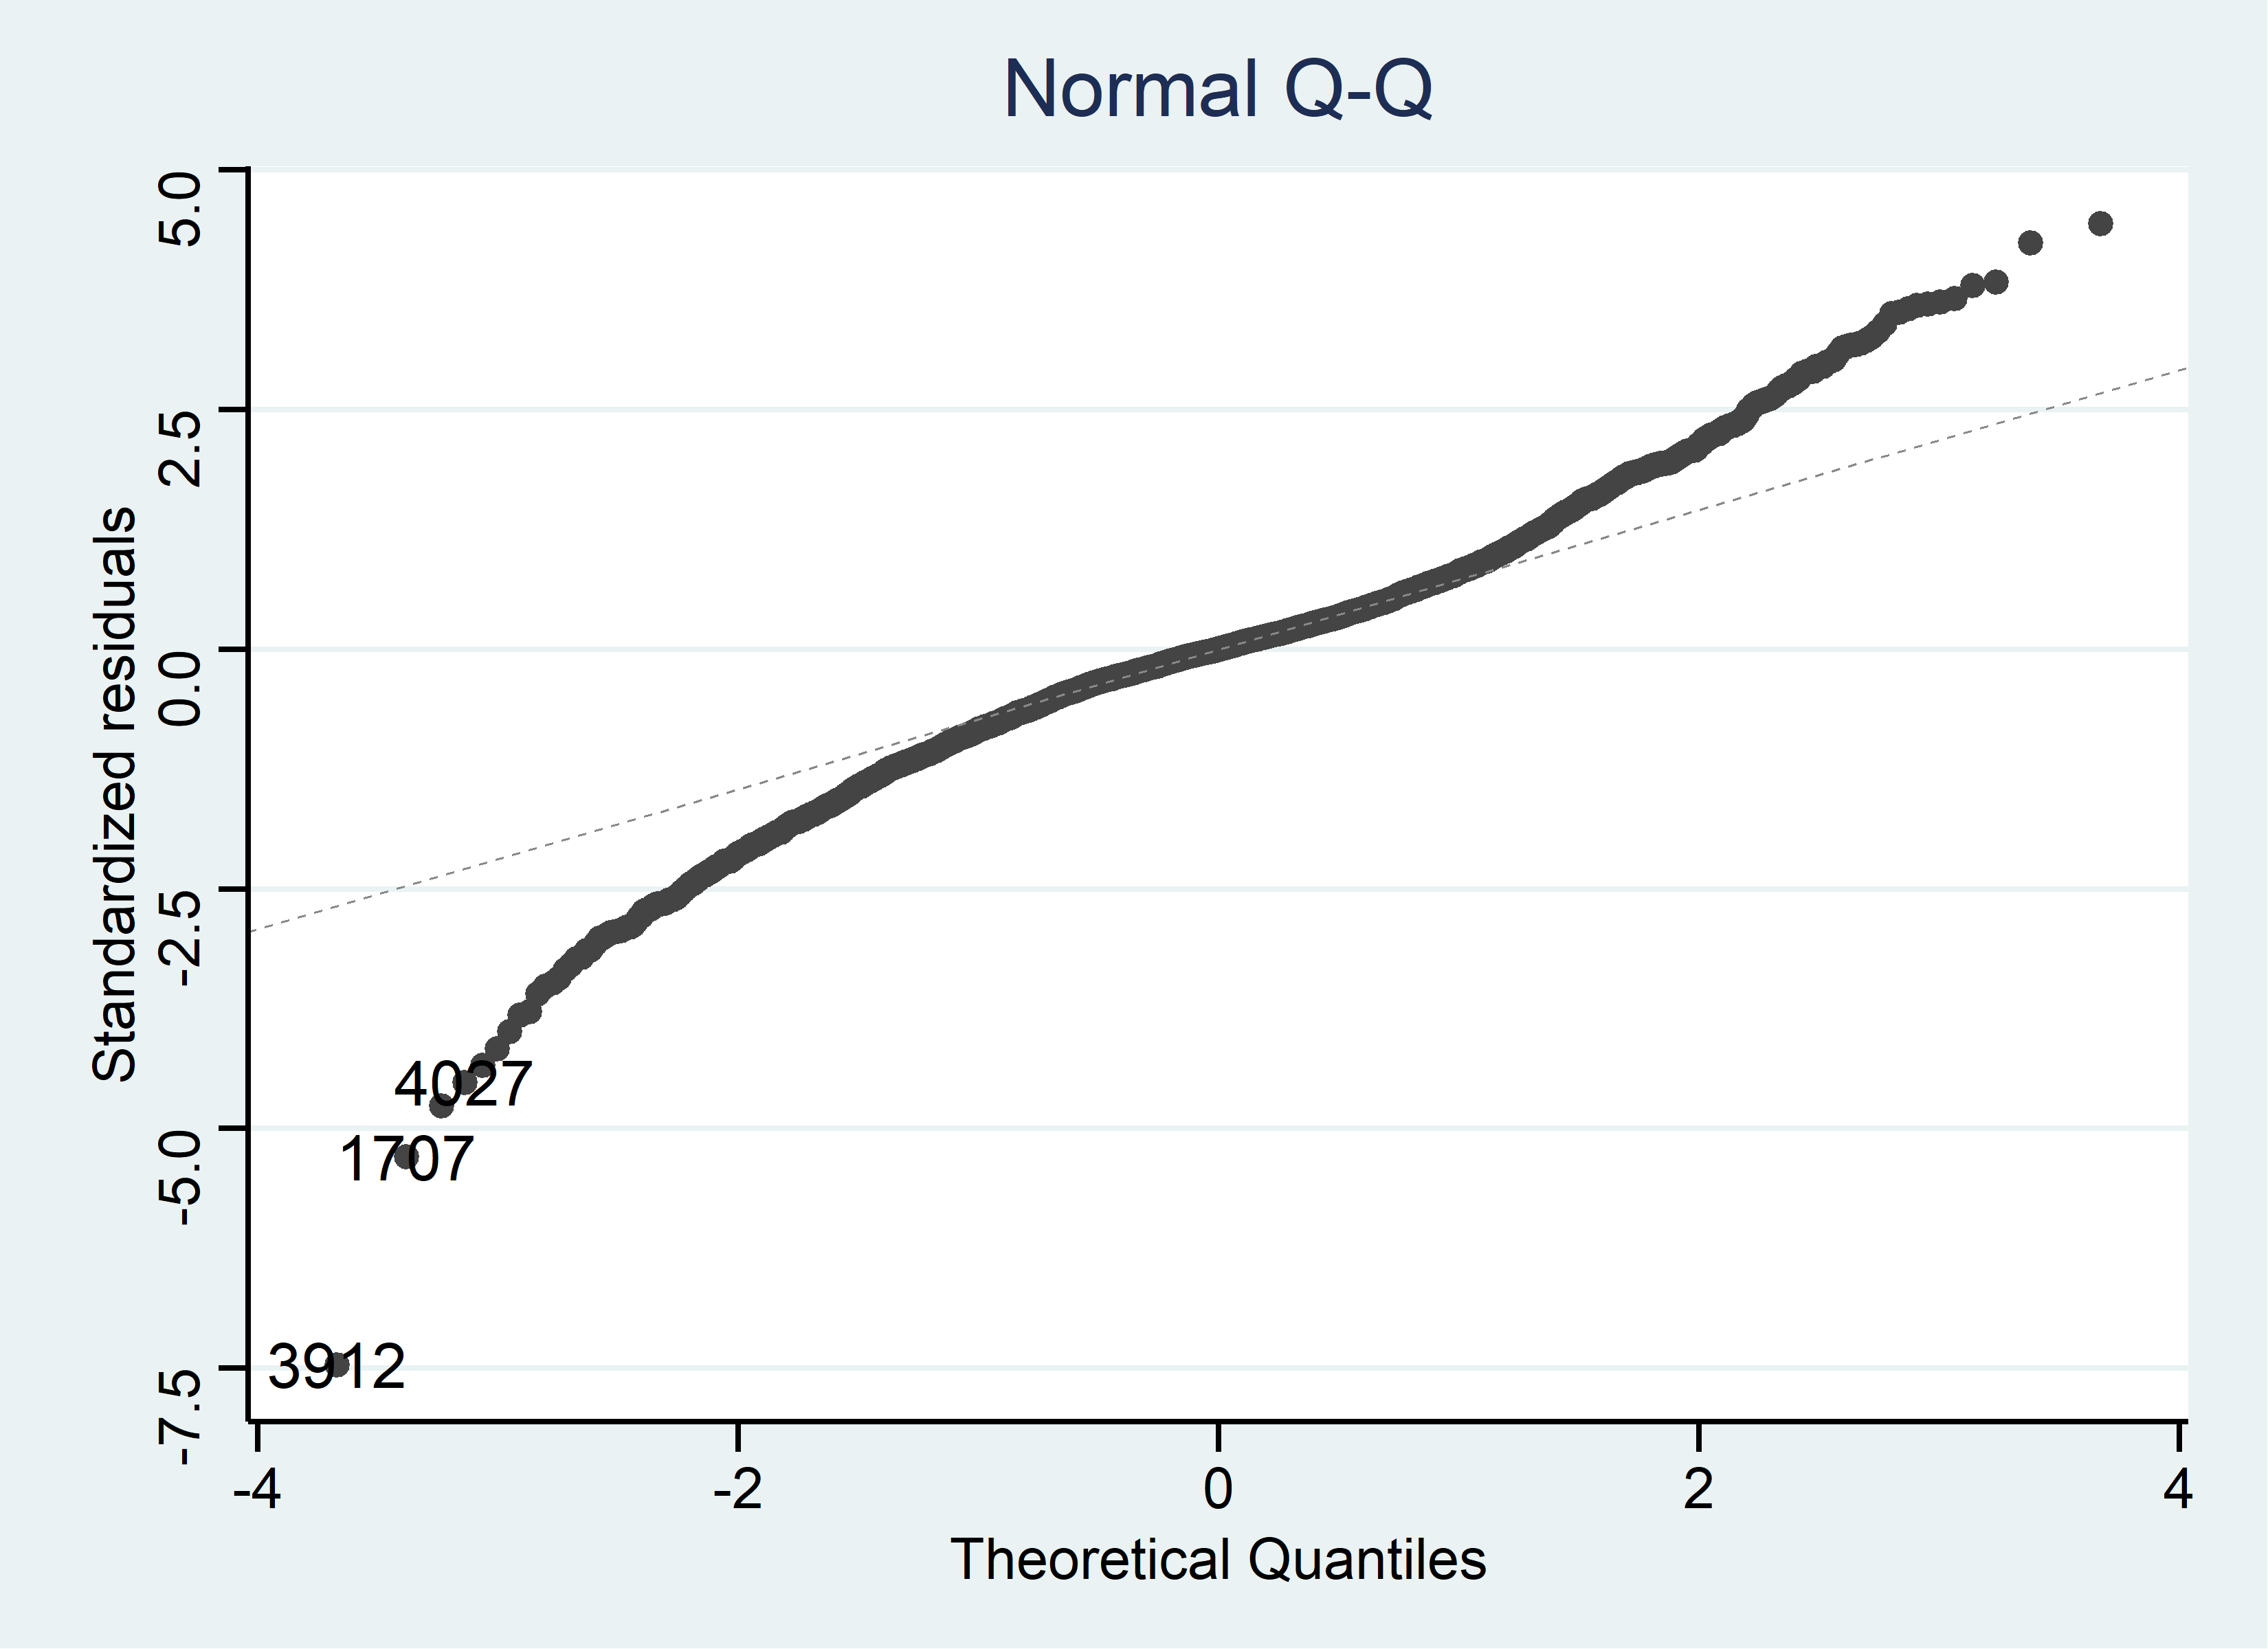
\includegraphics[height=4in,angle=0]{qq_mainmodel.png}
\end{center}
\end{figure}
\begin{figure}[!h]
\begin{center}
\caption{Histogram of bootstrapped coefficient (main model)}
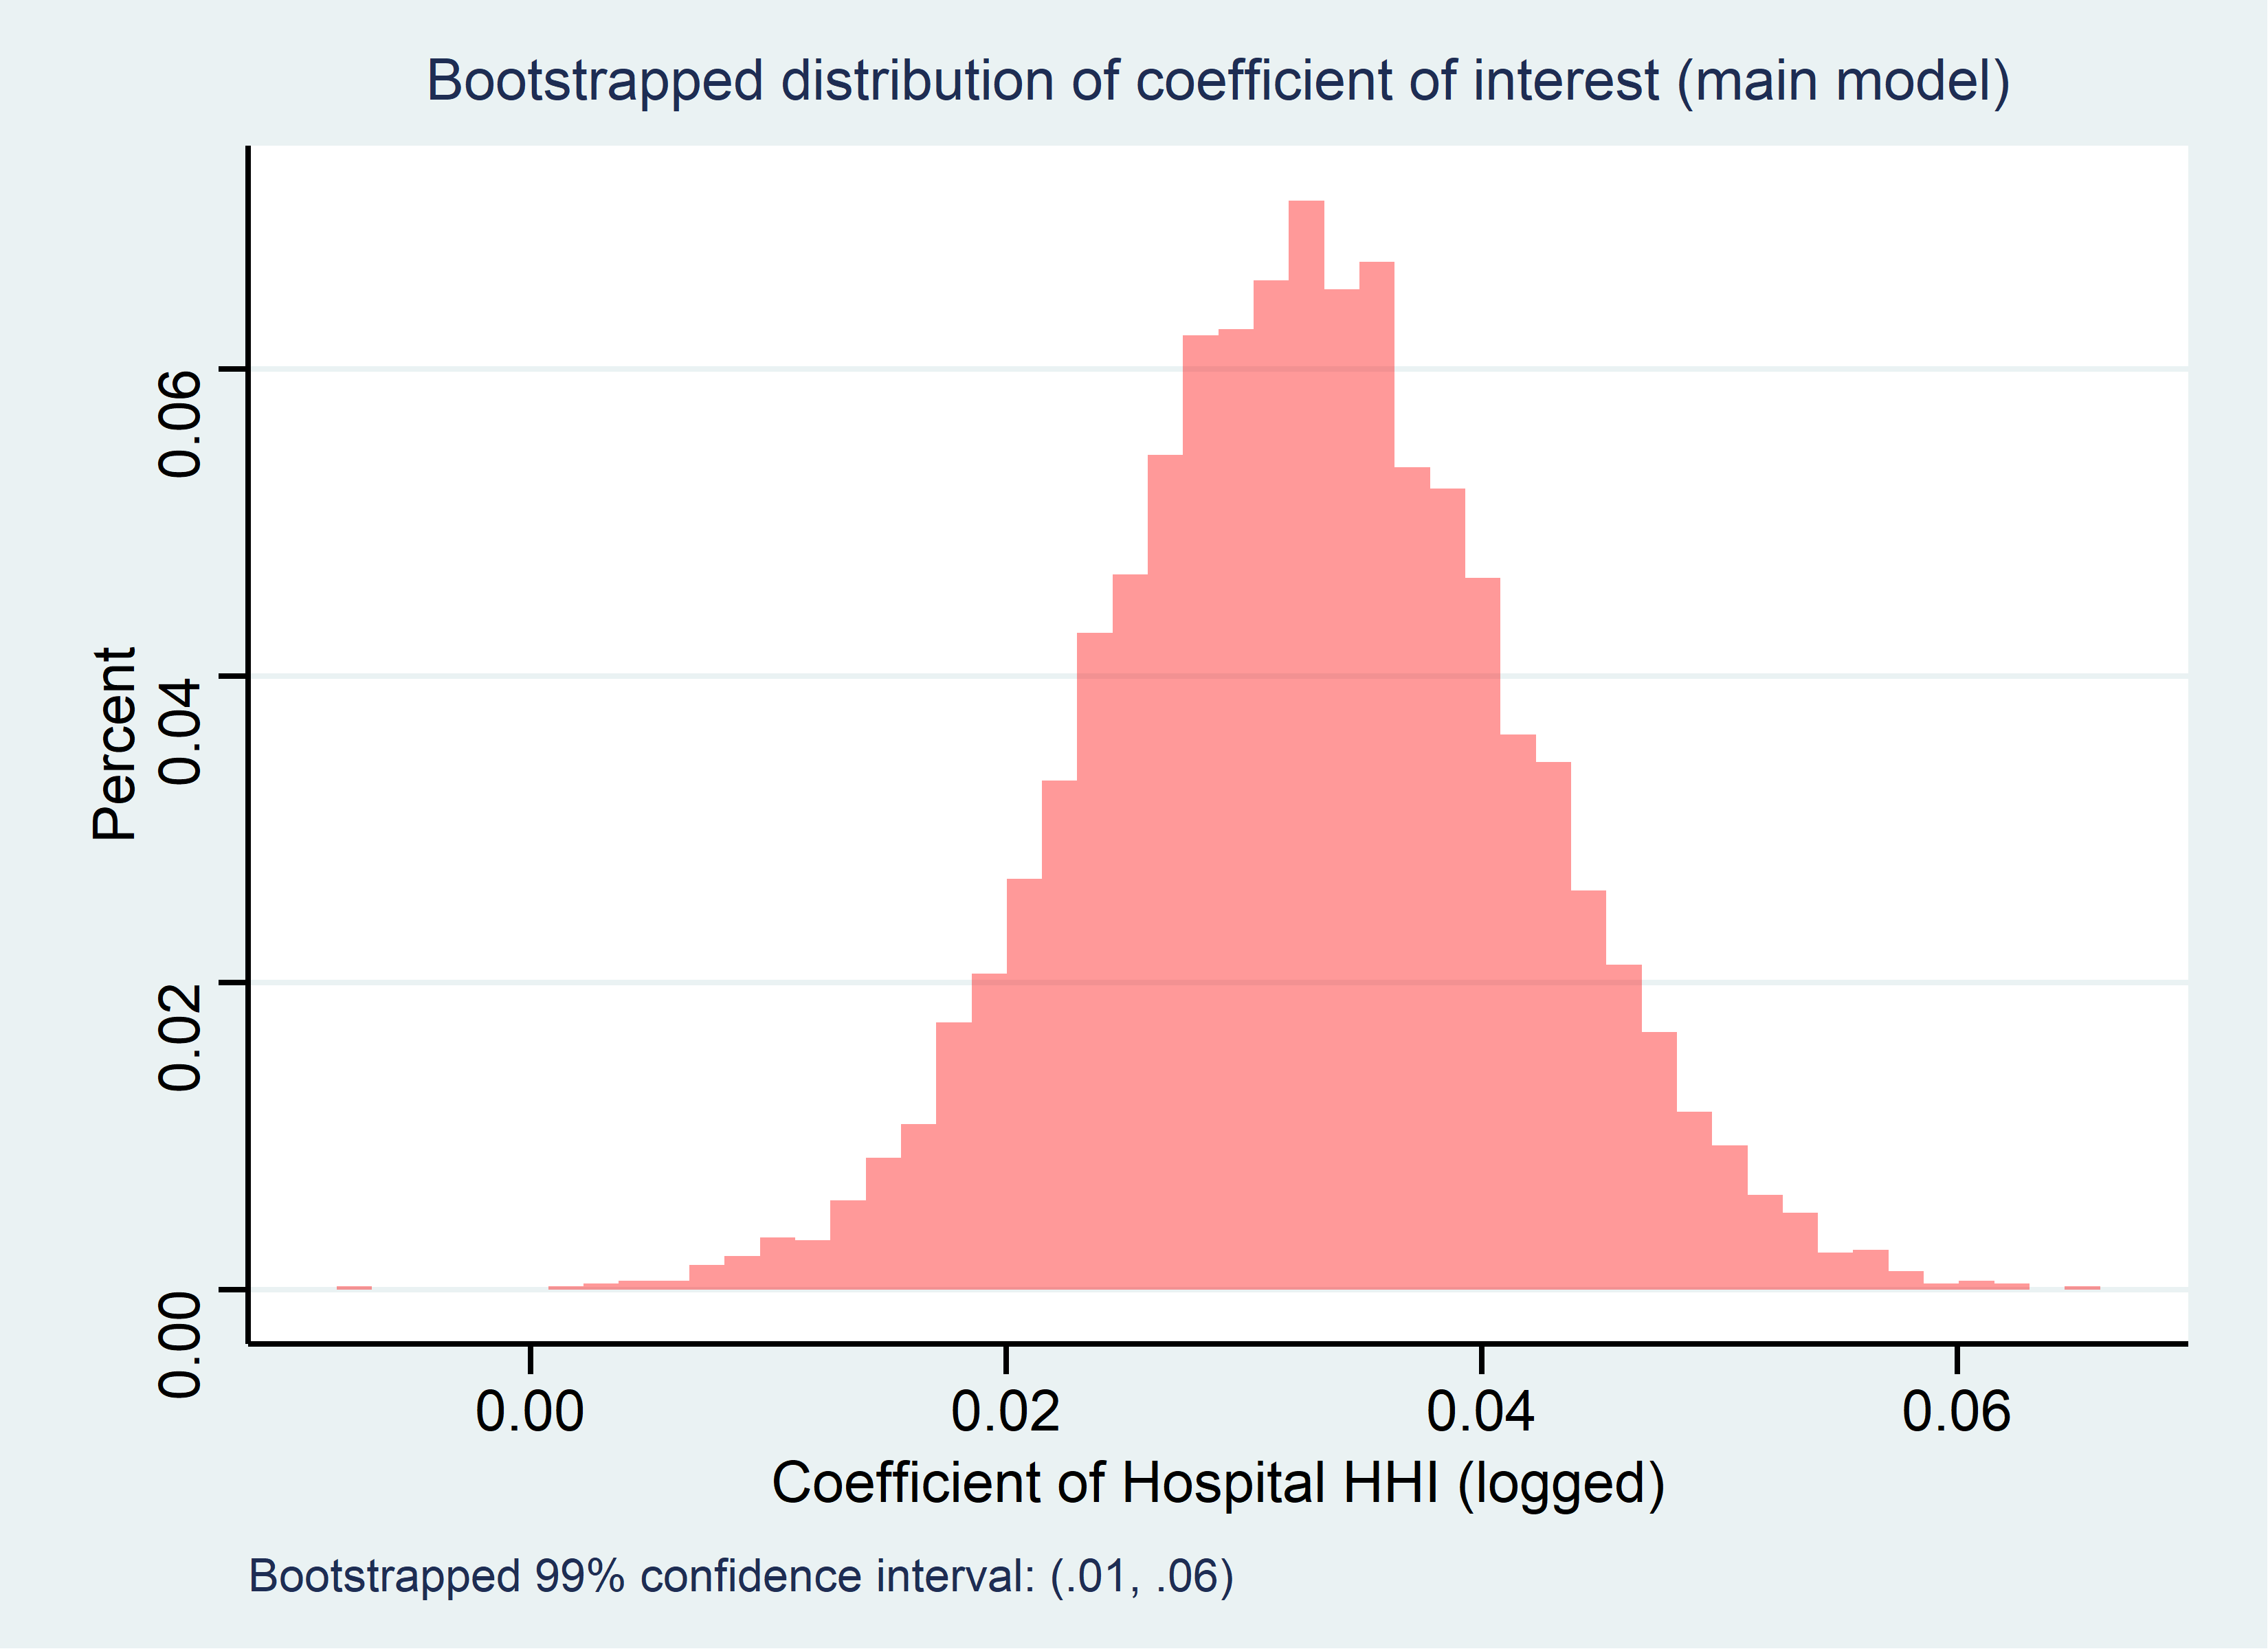
\includegraphics[height=4in,angle=0]{bootstrap_coef.png}
\end{center}
\end{figure}


\end{document}